%%%%%%%%%%%%%%%%%%%%%%%%%%%%%%%%%%%%%%%%%%%%%%%%%%%%%%%%%%%%%%%%%%%%%%%%%%%%%
%
%  System        : 
%  Module        : 
%  Object Name   : $RCSfile$
%  Revision      : $Revision$
%  Date          : $Date$
%  Author        : $Author$
%  Created By    : Robert Heller
%  Created       : Wed Apr 2 13:48:24 2025
%  Last Modified : <250405.1151>
%
%  Description 
%
%  Notes
%
%  History
% 
%%%%%%%%%%%%%%%%%%%%%%%%%%%%%%%%%%%%%%%%%%%%%%%%%%%%%%%%%%%%%%%%%%%%%%%%%%%%%
%
%    Copyright (C) 2025  Robert Heller D/B/A Deepwoods Software
%			51 Locke Hill Road
%			Wendell, MA 01379-9728
%
%    This program is free software; you can redistribute it and/or modify
%    it under the terms of the GNU General Public License as published by
%    the Free Software Foundation; either version 2 of the License, or
%    (at your option) any later version.
%
%    This program is distributed in the hope that it will be useful,
%    but WITHOUT ANY WARRANTY; without even the implied warranty of
%    MERCHANTABILITY or FITNESS FOR A PARTICULAR PURPOSE.  See the
%    GNU General Public License for more details.
%
%    You should have received a copy of the GNU General Public License
%    along with this program; if not, write to the Free Software
%    Foundation, Inc., 675 Mass Ave, Cambridge, MA 02139, USA.
%
% 
%
%%%%%%%%%%%%%%%%%%%%%%%%%%%%%%%%%%%%%%%%%%%%%%%%%%%%%%%%%%%%%%%%%%%%%%%%%%%%%


\documentclass[aspectratio=169]{beamer}

\mode<presentation>
{
  \usetheme{AnnArbor}
}
\usepackage[english]{babel}

\usepackage[latin1]{inputenc}

\usepackage{times}
\usepackage[T1]{fontenc}
\usepackage{url}
\usepackage{listings}
\lstset{language=Python,basicstyle=\footnotesize}
\usepackage{graphicx}
\title{Light up Embroidery Using a Gemma M0 and NeoPixels}
\author{Robert Heller}
\date{LaunchSpace}

%\subject{Video Presentation}

\usepackage{../rphpartpage}
\setbeamertemplate{part page}[video]
\AtBeginPart{\frame{\partpage}}
\begin{document}

\frame{\titlepage}

\part{Introduction}

\section{Who I am}
\begin{frame}[fragile]{Who I am}
My name is Robert Heller.  I have been writing computer programs for over 50
years.
\end{frame}
\section{What we will be making}
\begin{frame}[fragile]{What we will be making}
We will be creating a light up embroidering piece.  We will use a small, 
sewable microprocessor with some sewable lighting devices.
\end{frame}
\part{Materials and Tools}

\section{The electronics}
\frame{\tableofcontents[hideothersubsections,sectionstyle=show/hide]}

\subsection{The microprocessor: Gemma M0}
\begin{frame}[fragile]{The microprocessor: Gemma M0}
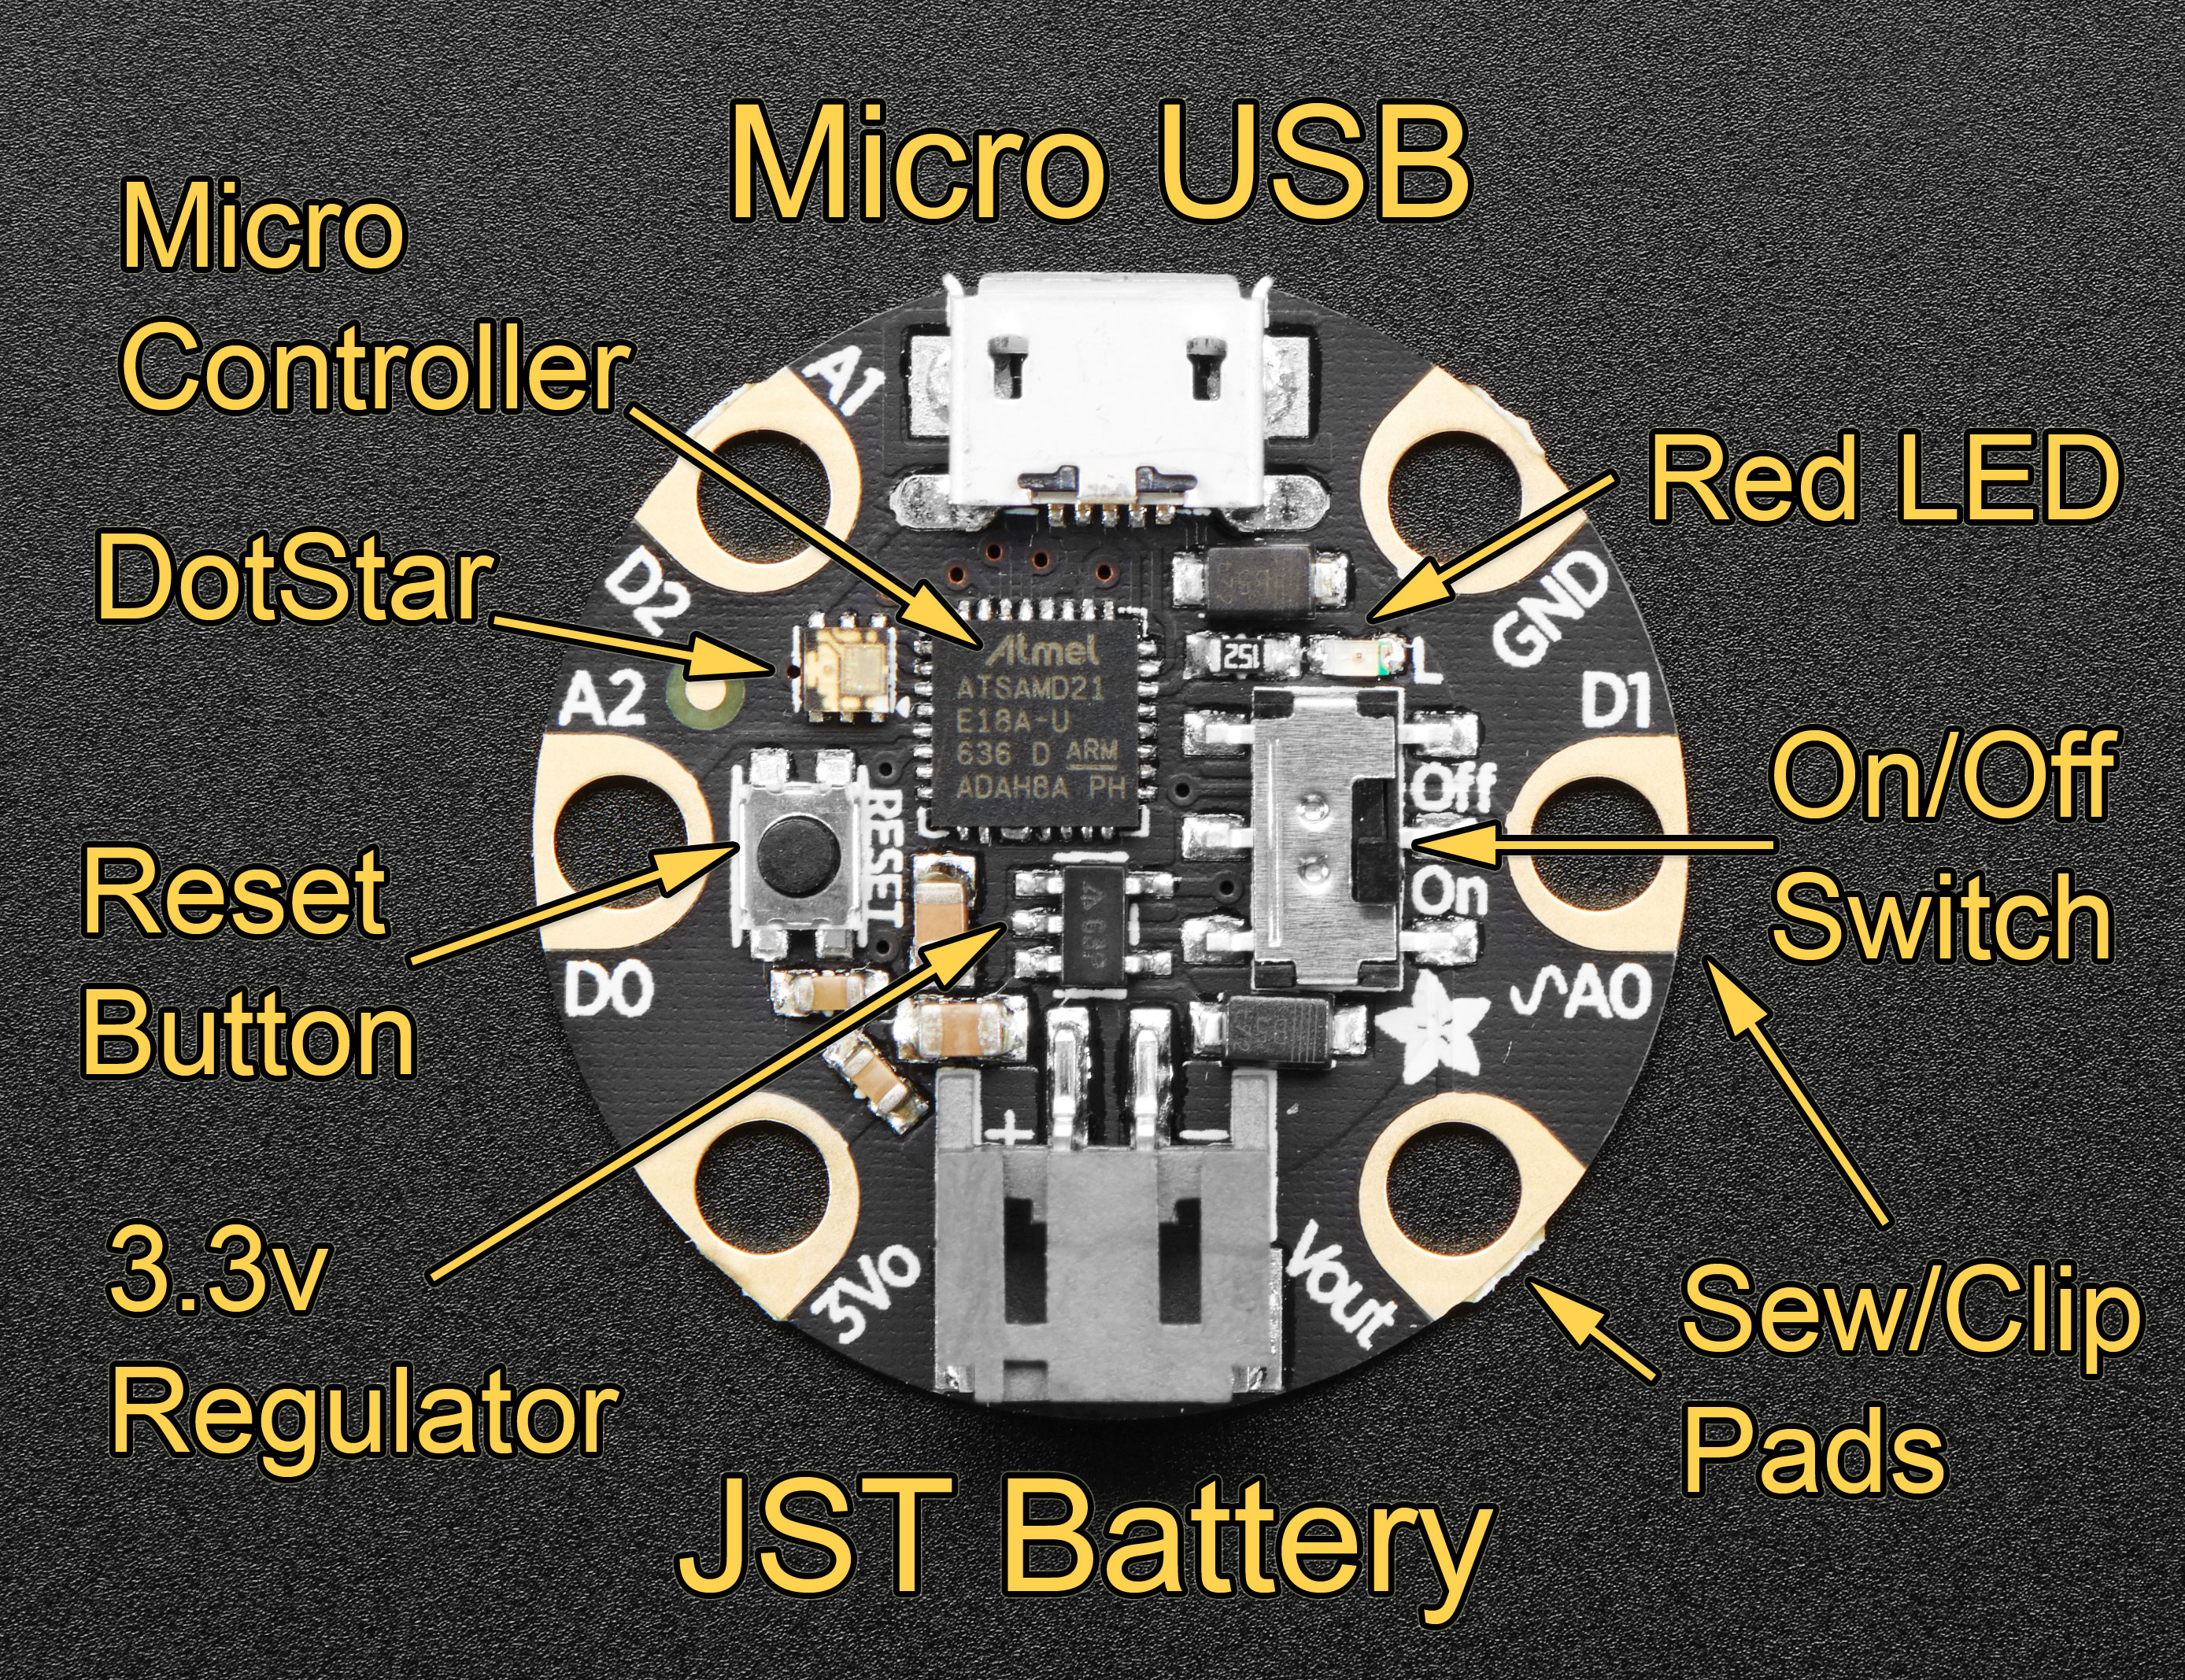
\includegraphics[height=2.75in]{gemma_guide.jpg}
\end{frame}
\begin{frame}[fragile]{Gemma M0 pins}
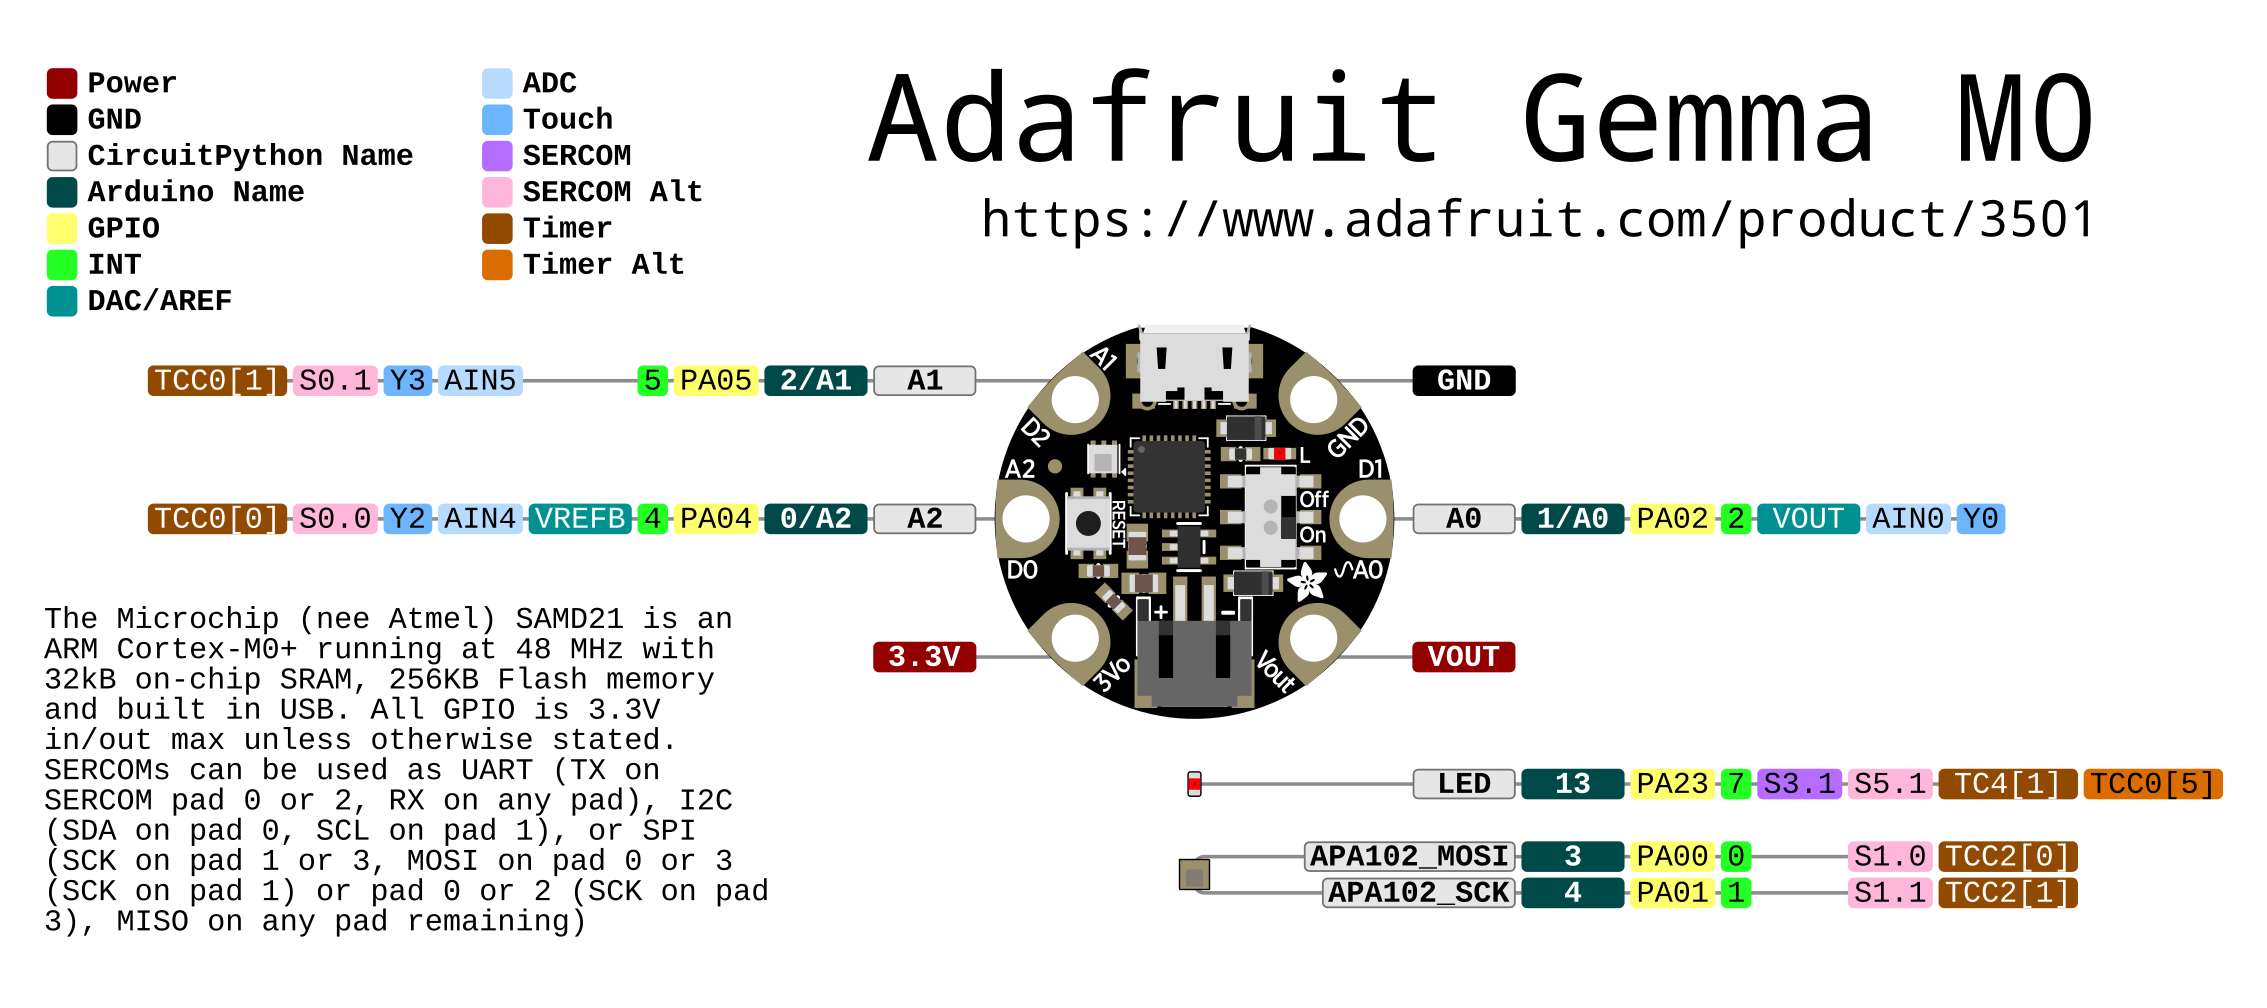
\includegraphics[width=5in]{adafruit_gemma_Adafruit_GEMMA_M0_pinout.png}
\end{frame}
\subsection{The NeoPixel}
\begin{frame}[fragile]{The NeoPixel}
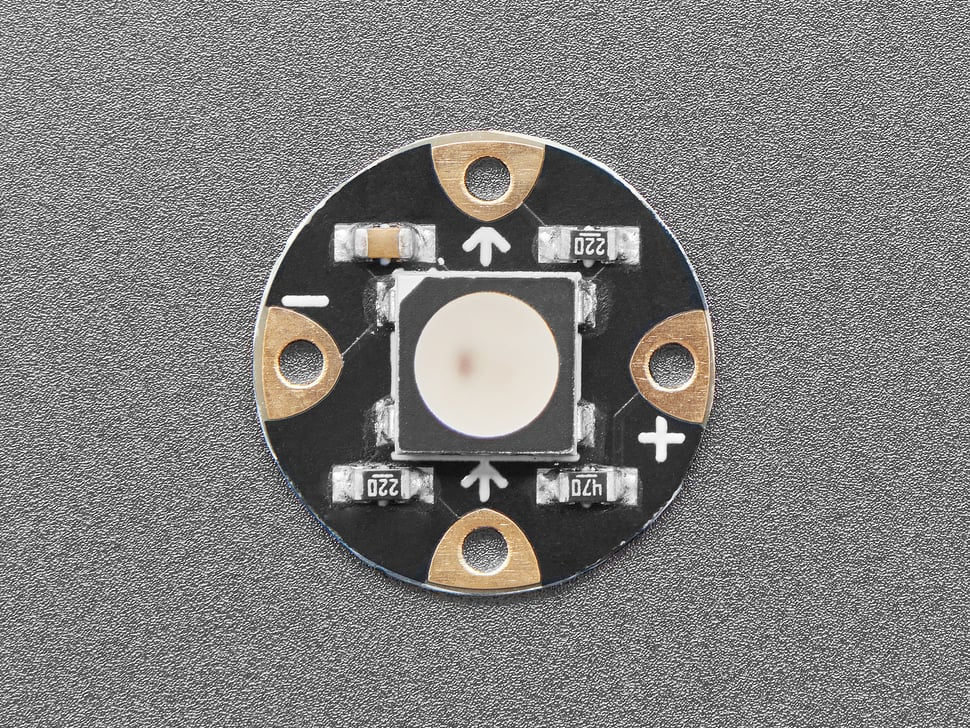
\includegraphics[height=2.75in]{FloraNeoPixel.jpg}
\end{frame}
\subsection{Snaps}
\begin{frame}[fragile]{Snaps}
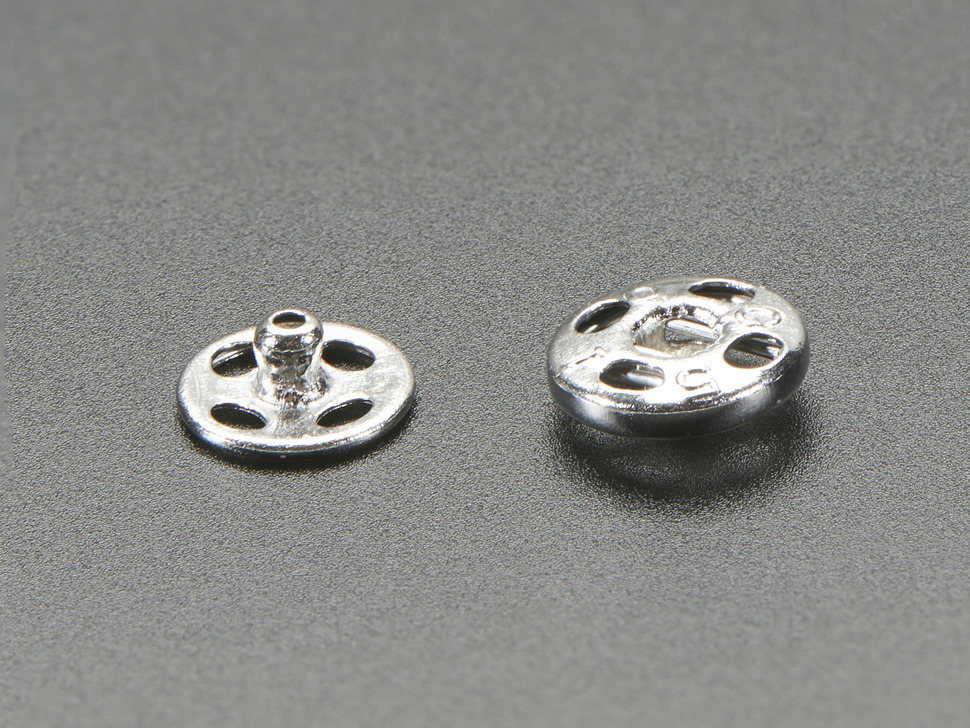
\includegraphics[height=2.75in]{snap.jpg}
\end{frame}
\subsection{Conductive Thread}
\begin{frame}[fragile]{Conductive Thread}
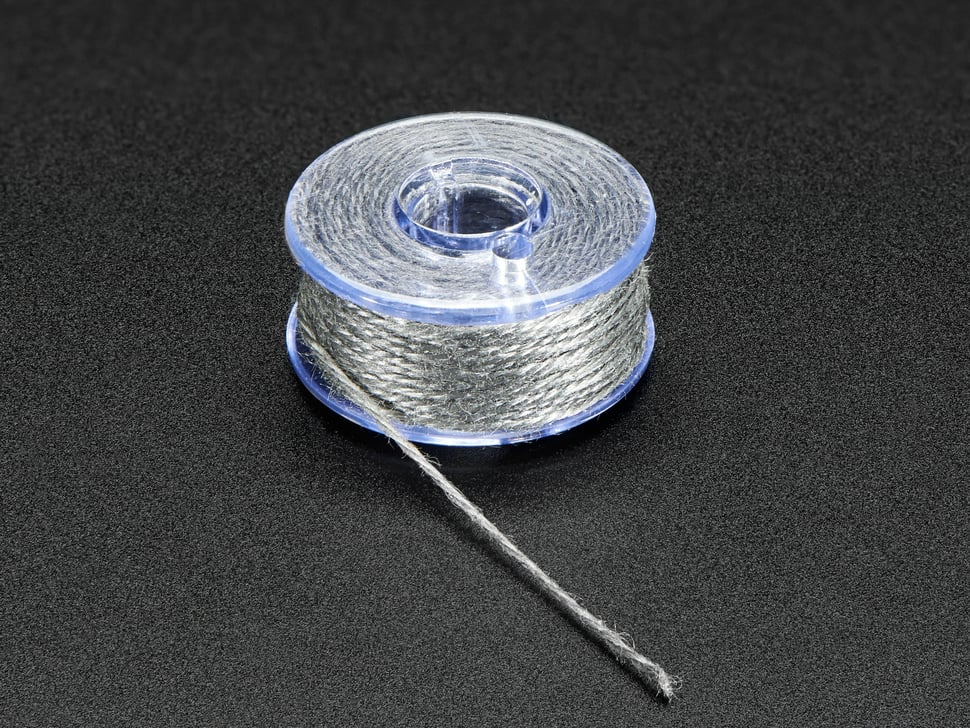
\includegraphics[height=2.75in]{conductivethread.jpg}
\end{frame}
\subsection{Battery Holder and extension cable}
\begin{frame}[fragile]{Battery Holder}
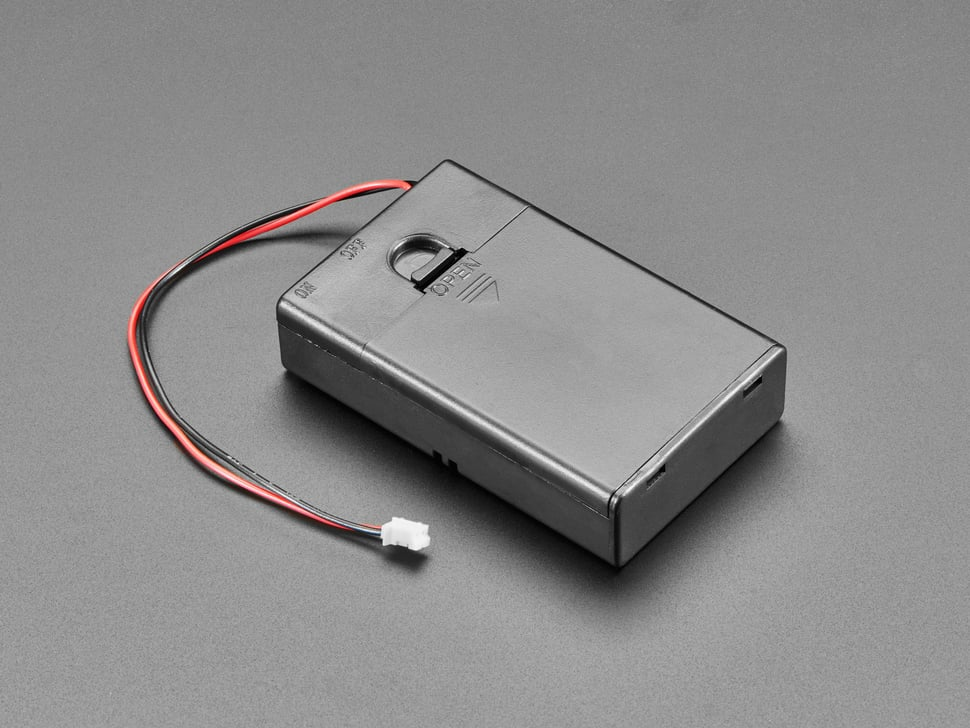
\includegraphics[height=2.75in]{BatteryHolder.jpg}
\end{frame}
\begin{frame}[fragile]{Extension Cable}
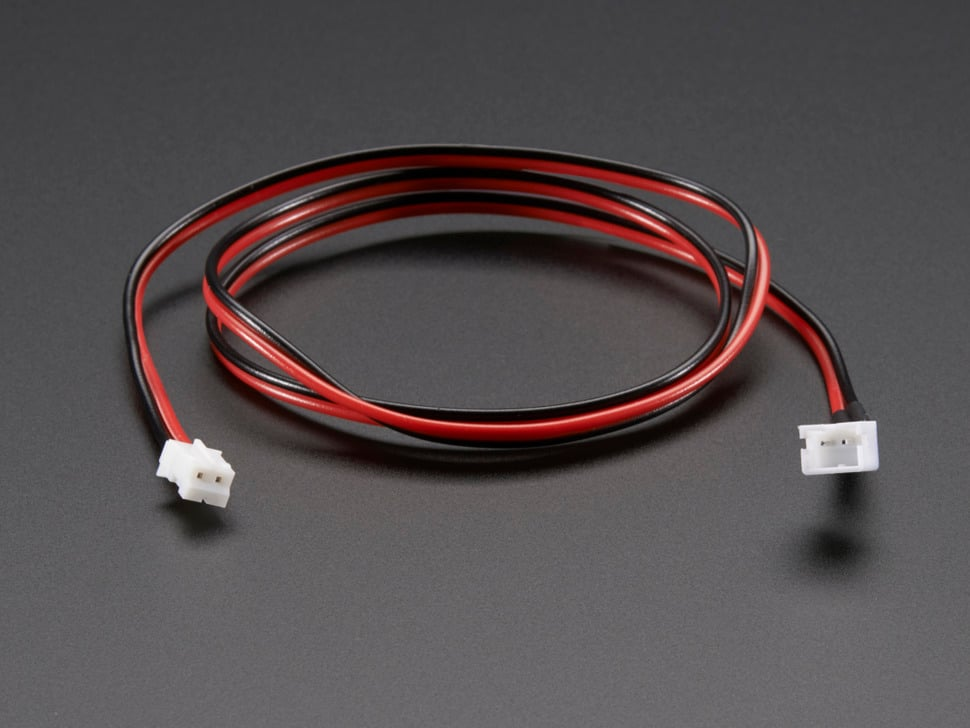
\includegraphics[height=2.75in]{ExtenssionCable.jpg}
\end{frame}
\subsection{USB Cable}
\begin{frame}[fragile]{USB Cable}
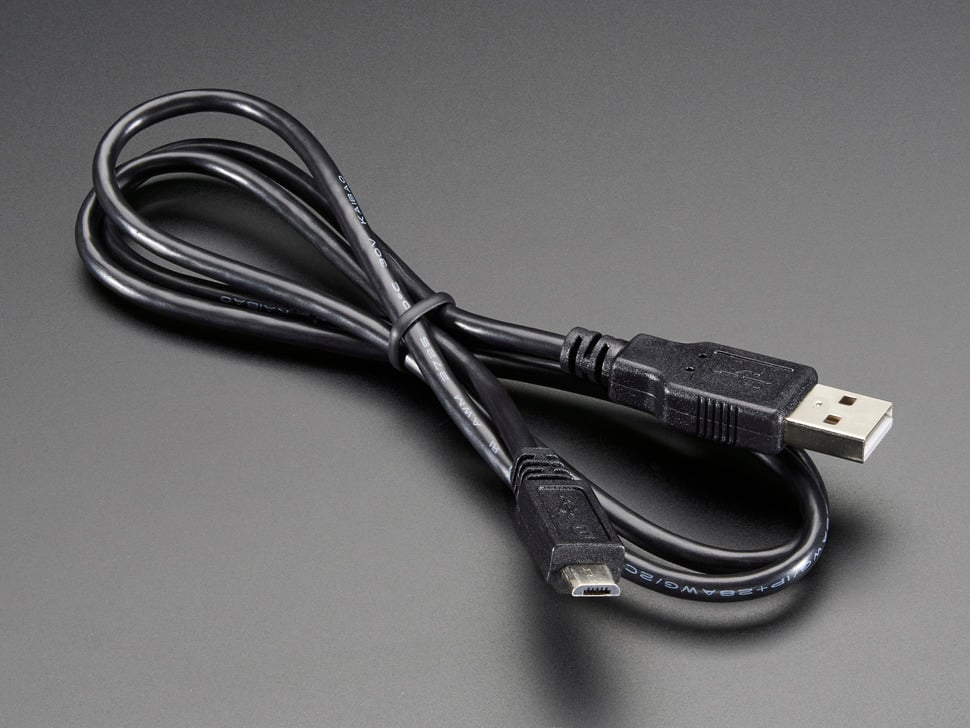
\includegraphics[width=4in]{USBCable.jpg}
\end{frame}
\section{Other materials}
\frame{\tableofcontents[hideothersubsections,sectionstyle=show/hide]}
\subsection{Embroidery Thread}
\begin{frame}[fragile]{Embroidery Thread}
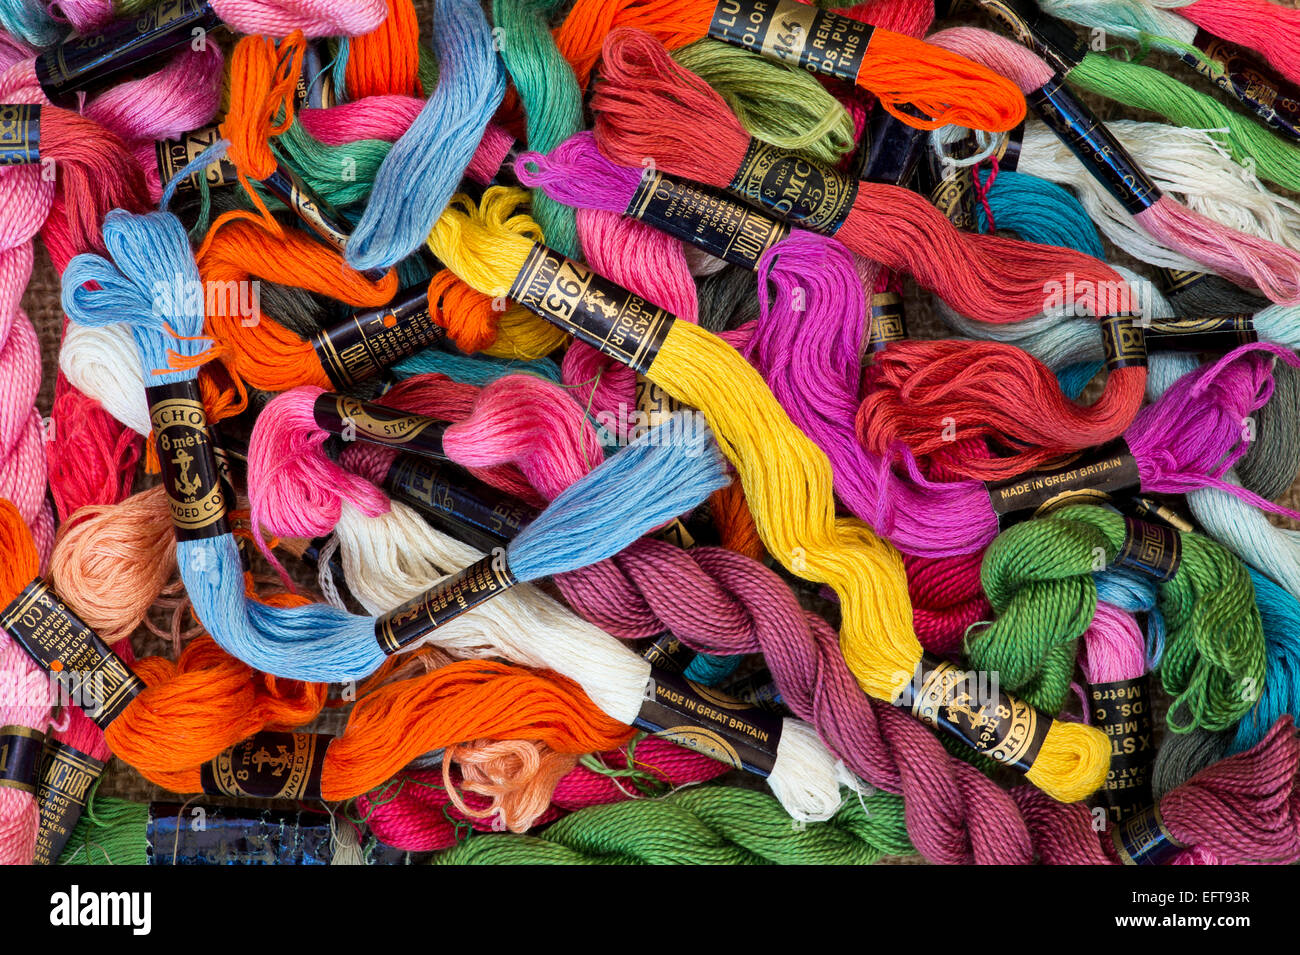
\includegraphics[height=2.75in]{embroiderythreads.jpg}
\end{frame}
\subsection{Fabric Scraps}
\begin{frame}[fragile]{Fabric Scraps}
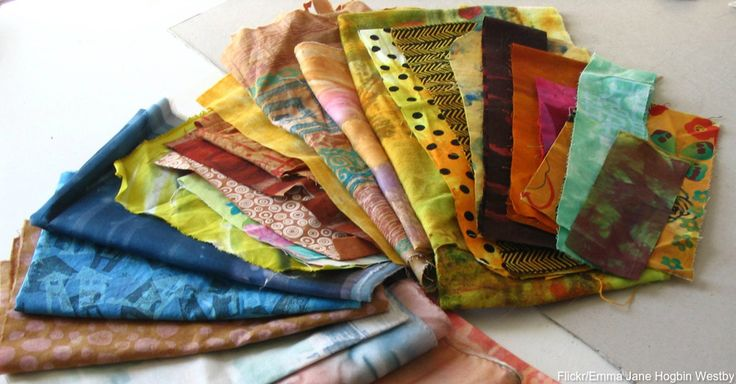
\includegraphics[height=2.75in]{FabricScraps.jpg}
\end{frame}
\subsection{Clear Nail Polish}
\begin{frame}[fragile]{Clear Nail Polish}

\includegraphics[height=2.75in]{ClearNailPolish.jpeg}
\end{frame}
\section{The Tools}
\frame{\tableofcontents[hideothersubsections,sectionstyle=show/hide]}
\subsection{Needles}
\begin{frame}[fragile]{Needles}
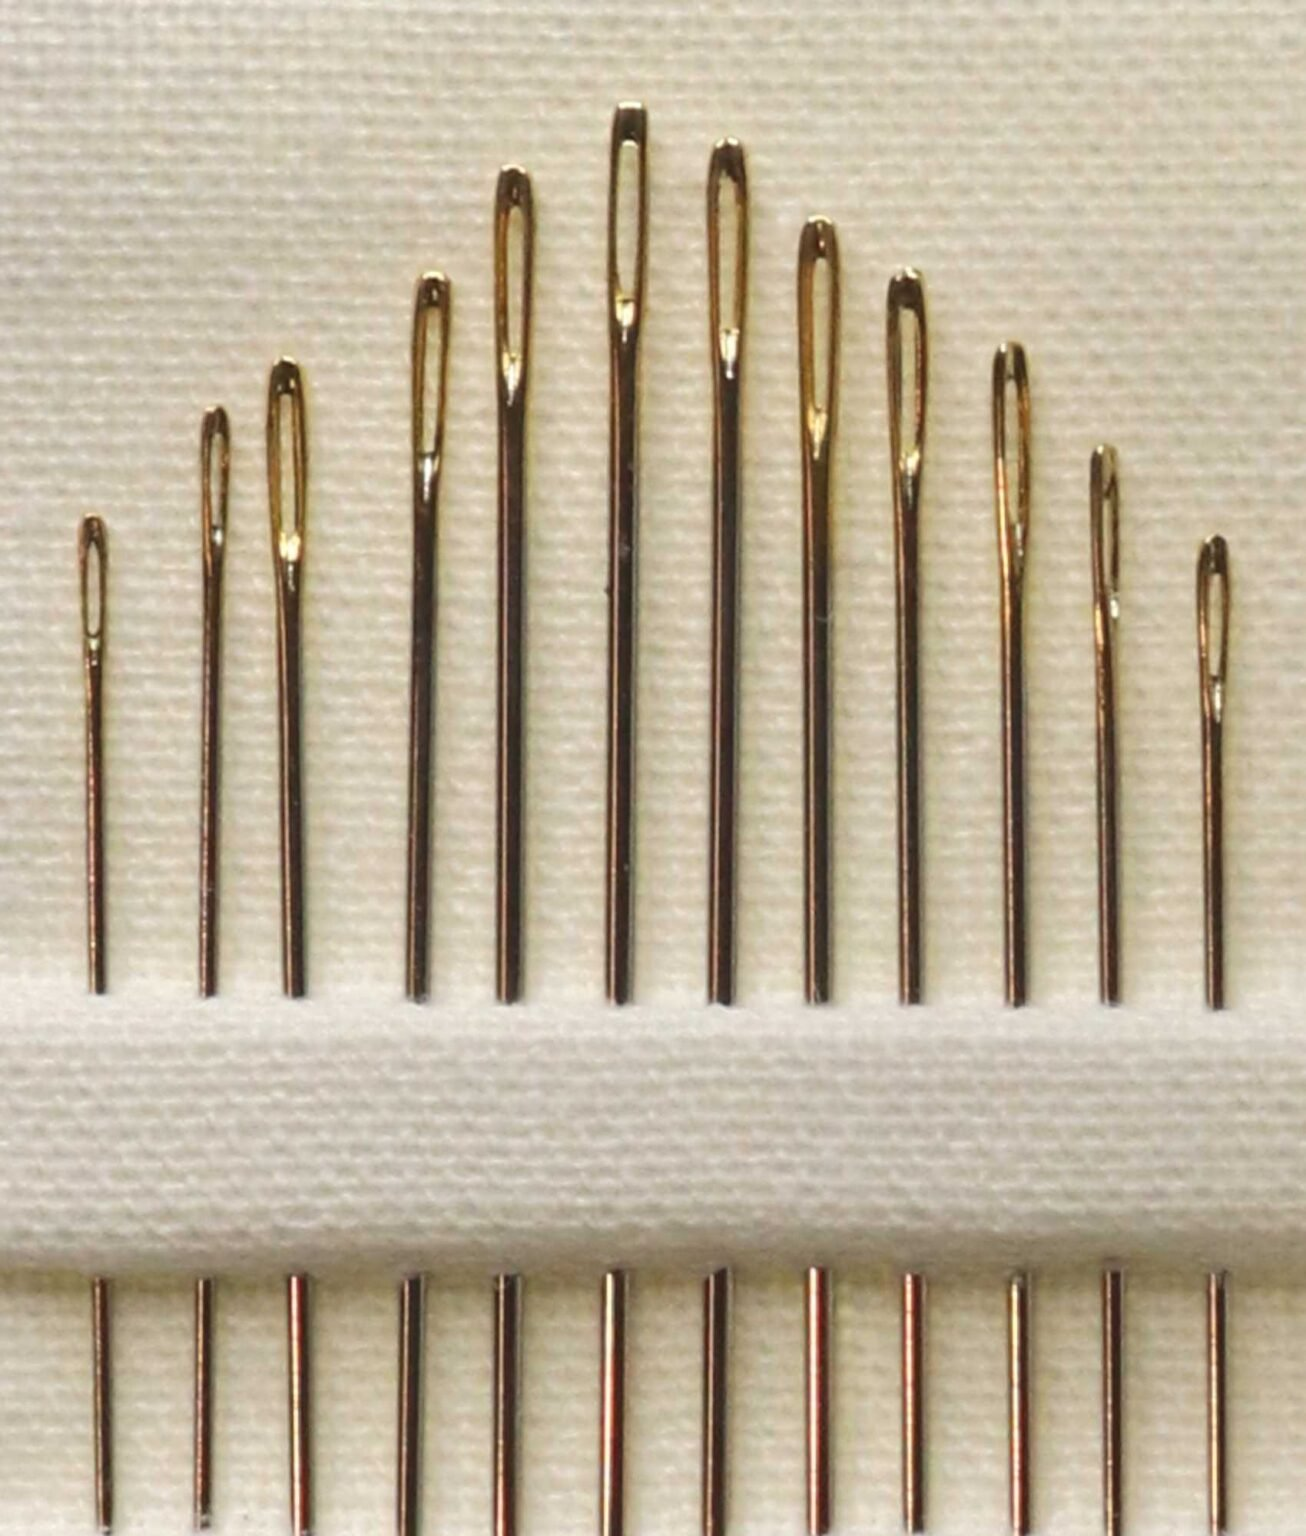
\includegraphics[height=2.75in]{Needles.jpg}
\end{frame}
\subsection{Scissors}
\begin{frame}[fragile]{Scissors}
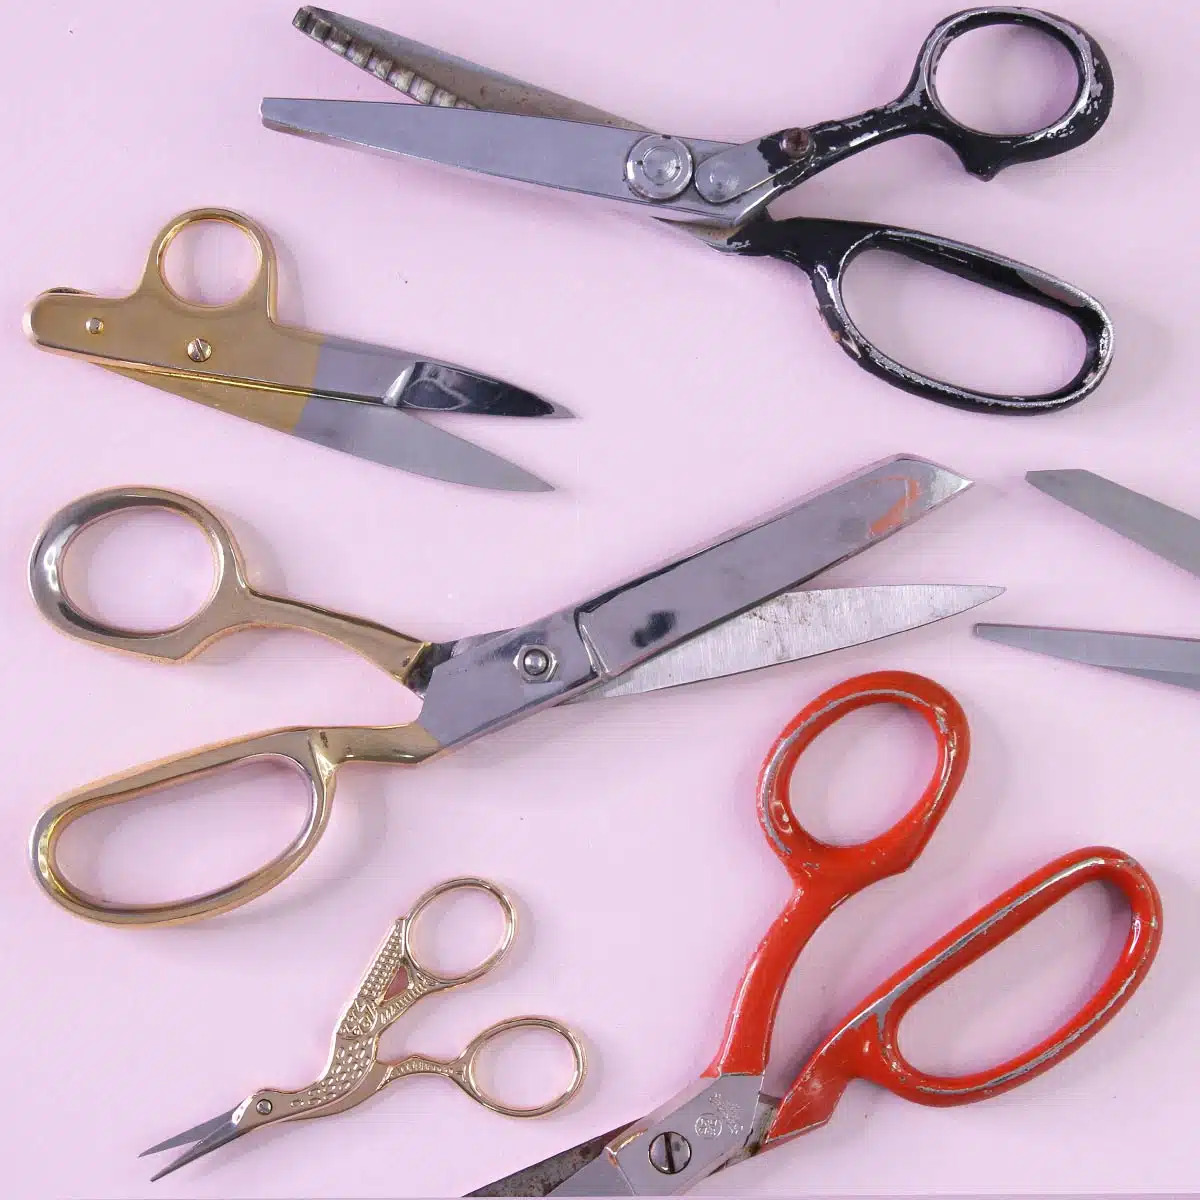
\includegraphics[height=2.75in]{Scissors.jpg}
\end{frame}
\subsection{Embroidery hoop}
\begin{frame}[fragile]{Embroidery hoop}
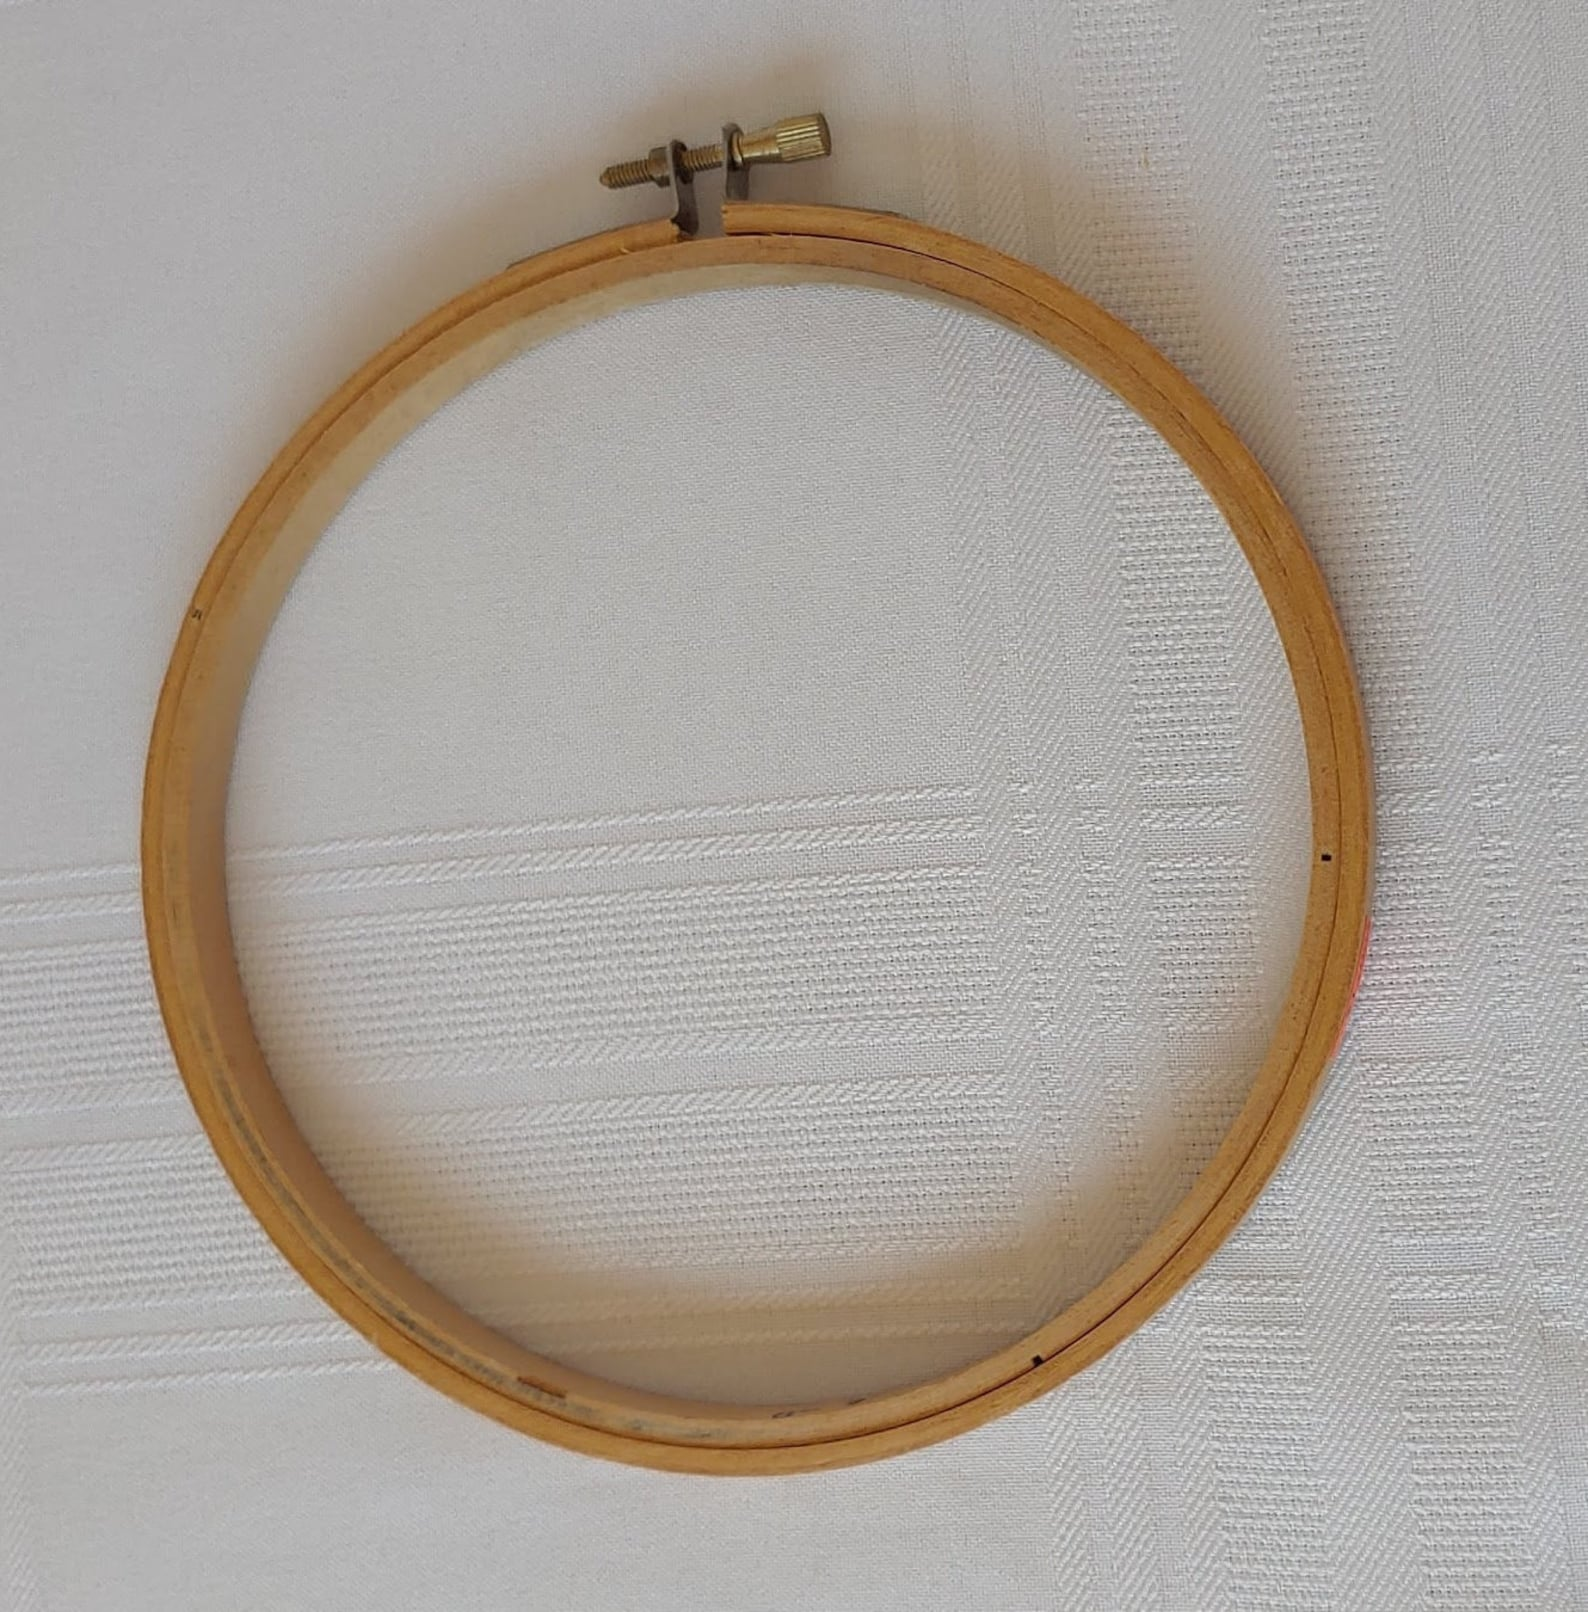
\includegraphics[height=2.75in]{Embroideryhoop.jpg}
\end{frame}
\subsection{Fabric markers and tailor's chalk}
\begin{frame}[fragile]{Fabric markers and tailor's chalk}
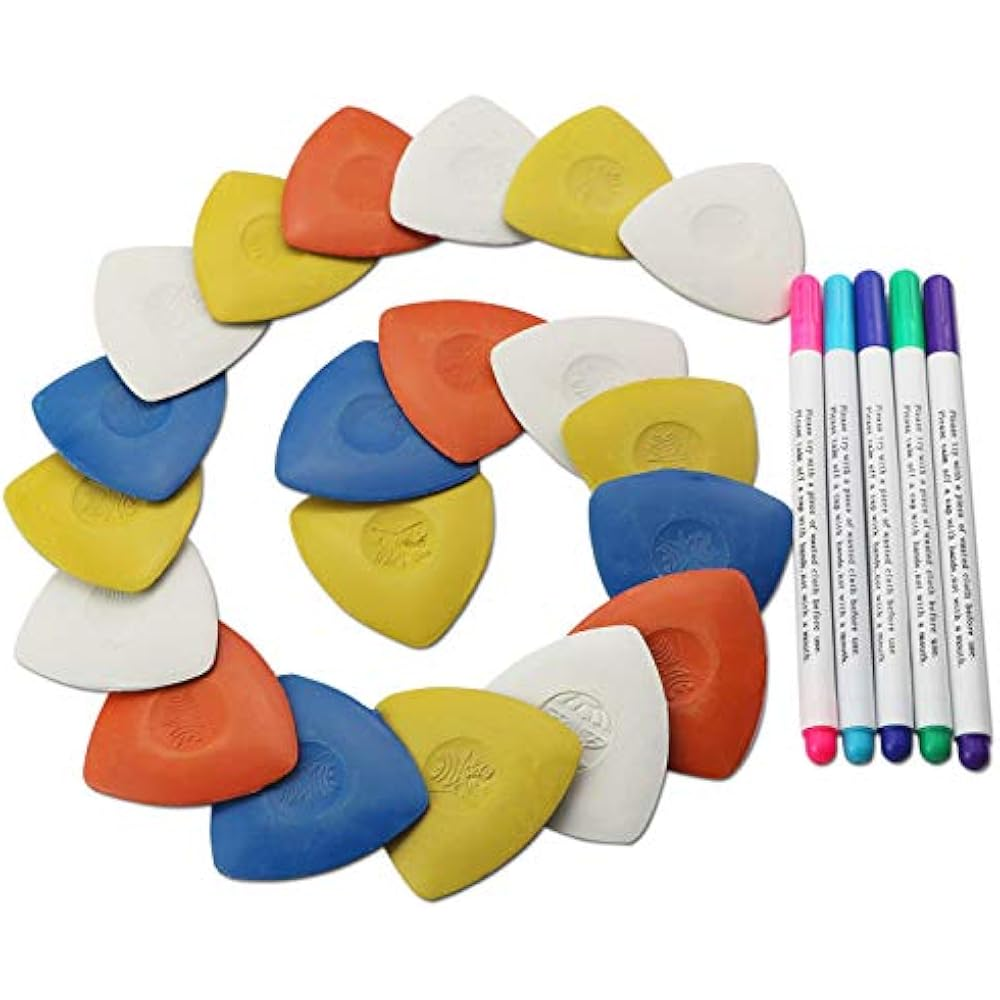
\includegraphics[height=2.75in]{Fabricmarkerstailorschalk.jpg}
\end{frame}
\subsection{Paper and pencils}
\begin{frame}[fragile]{Paper and pencils}

\includegraphics[height=2.75in]{Paperandpencils.jpg}
\end{frame}
\part{Designing the Embroidery}
\begin{frame}[fragile]{Bioluminescence-Deep-Sea-Fish}

\includegraphics[height=2.75in]{Bioluminescence-Deep-Sea-Fish-777x518.jpg}
\end{frame}
\begin{frame}[fragile]{Bioluminescence-Fireflies}
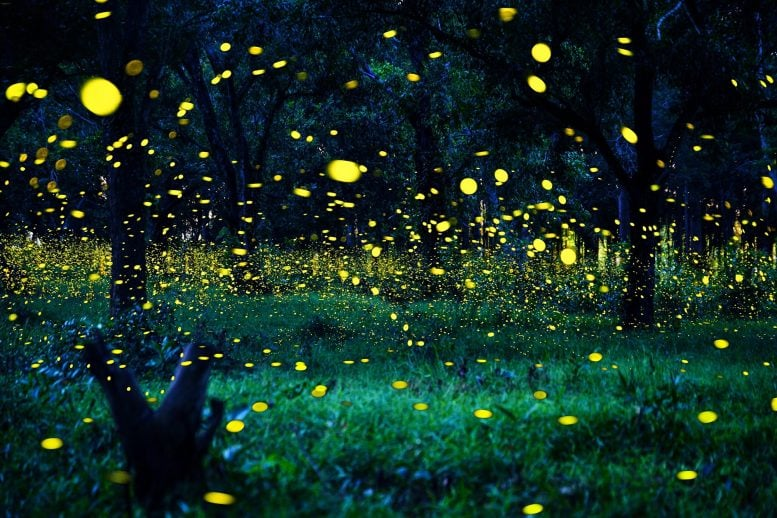
\includegraphics[height=2.75in]{Bioluminescence-Fireflies-777x518.jpg}
\end{frame}
\begin{frame}[fragile]{Orion}
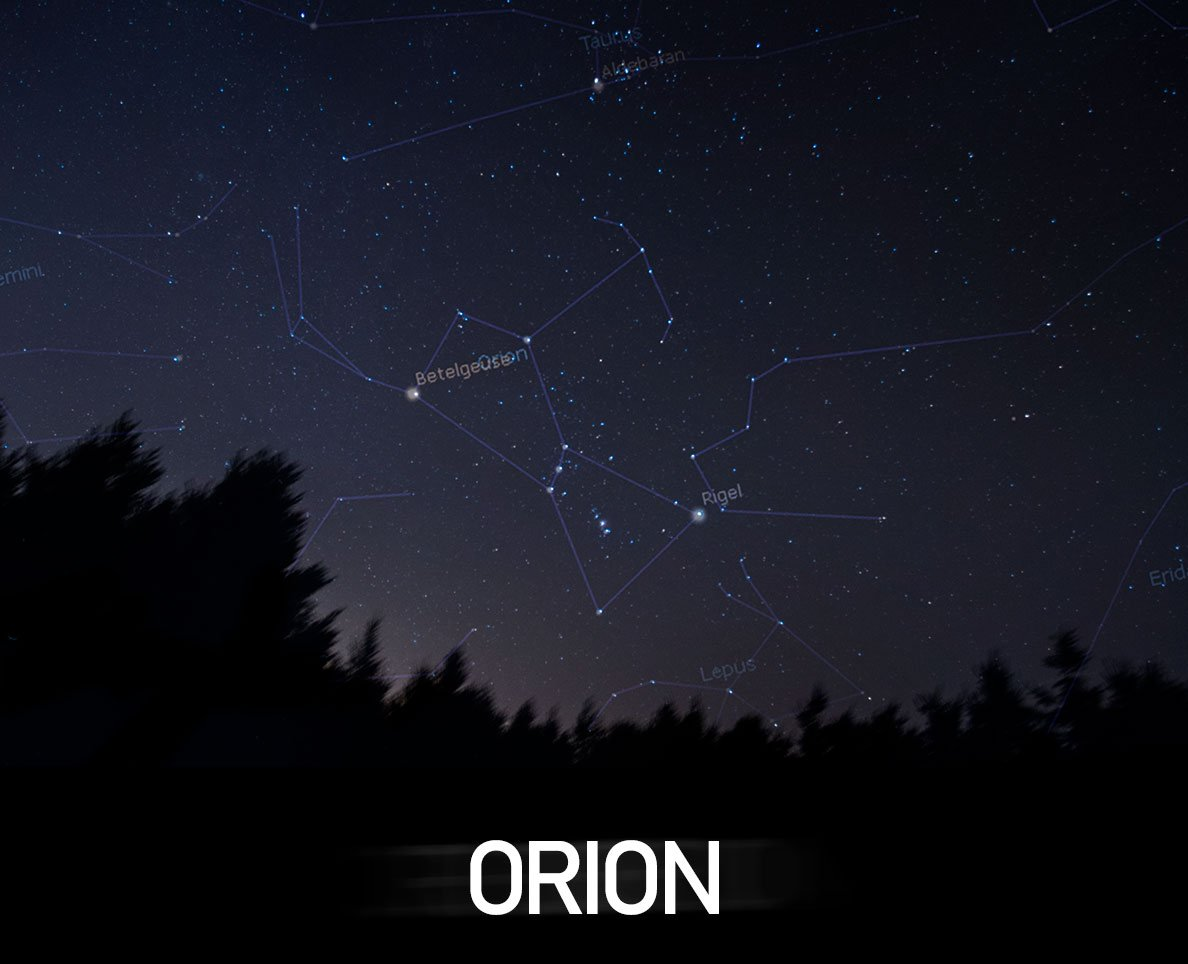
\includegraphics[height=2.75in]{orion.jpg}
\end{frame}
\begin{frame}[fragile]{Jupiter and moons}
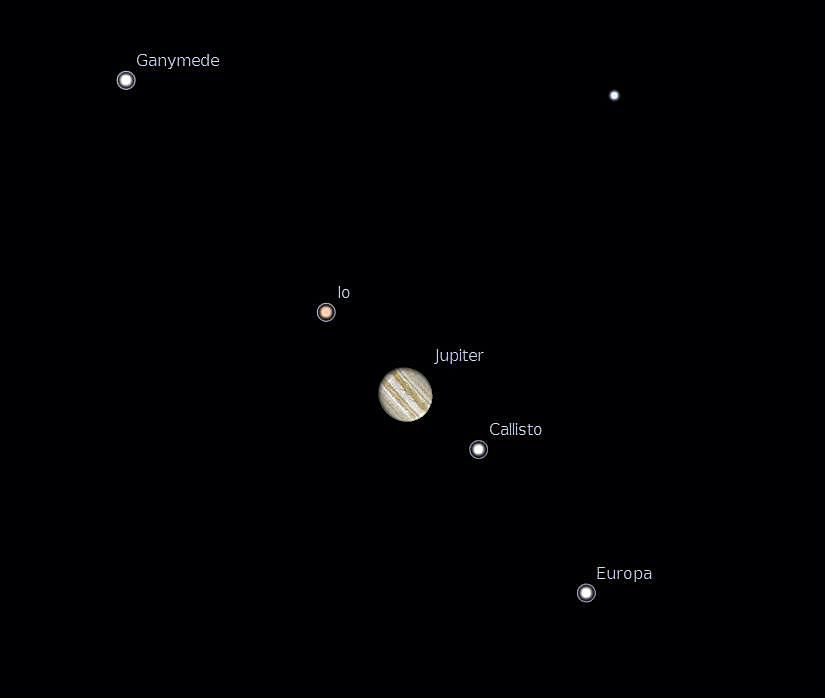
\includegraphics[height=2.75in]{Jupiter-and-moons-58b82f8c3df78c060e64eb8b.jpg}
\end{frame}
\begin{frame}[fragile]{Comet}
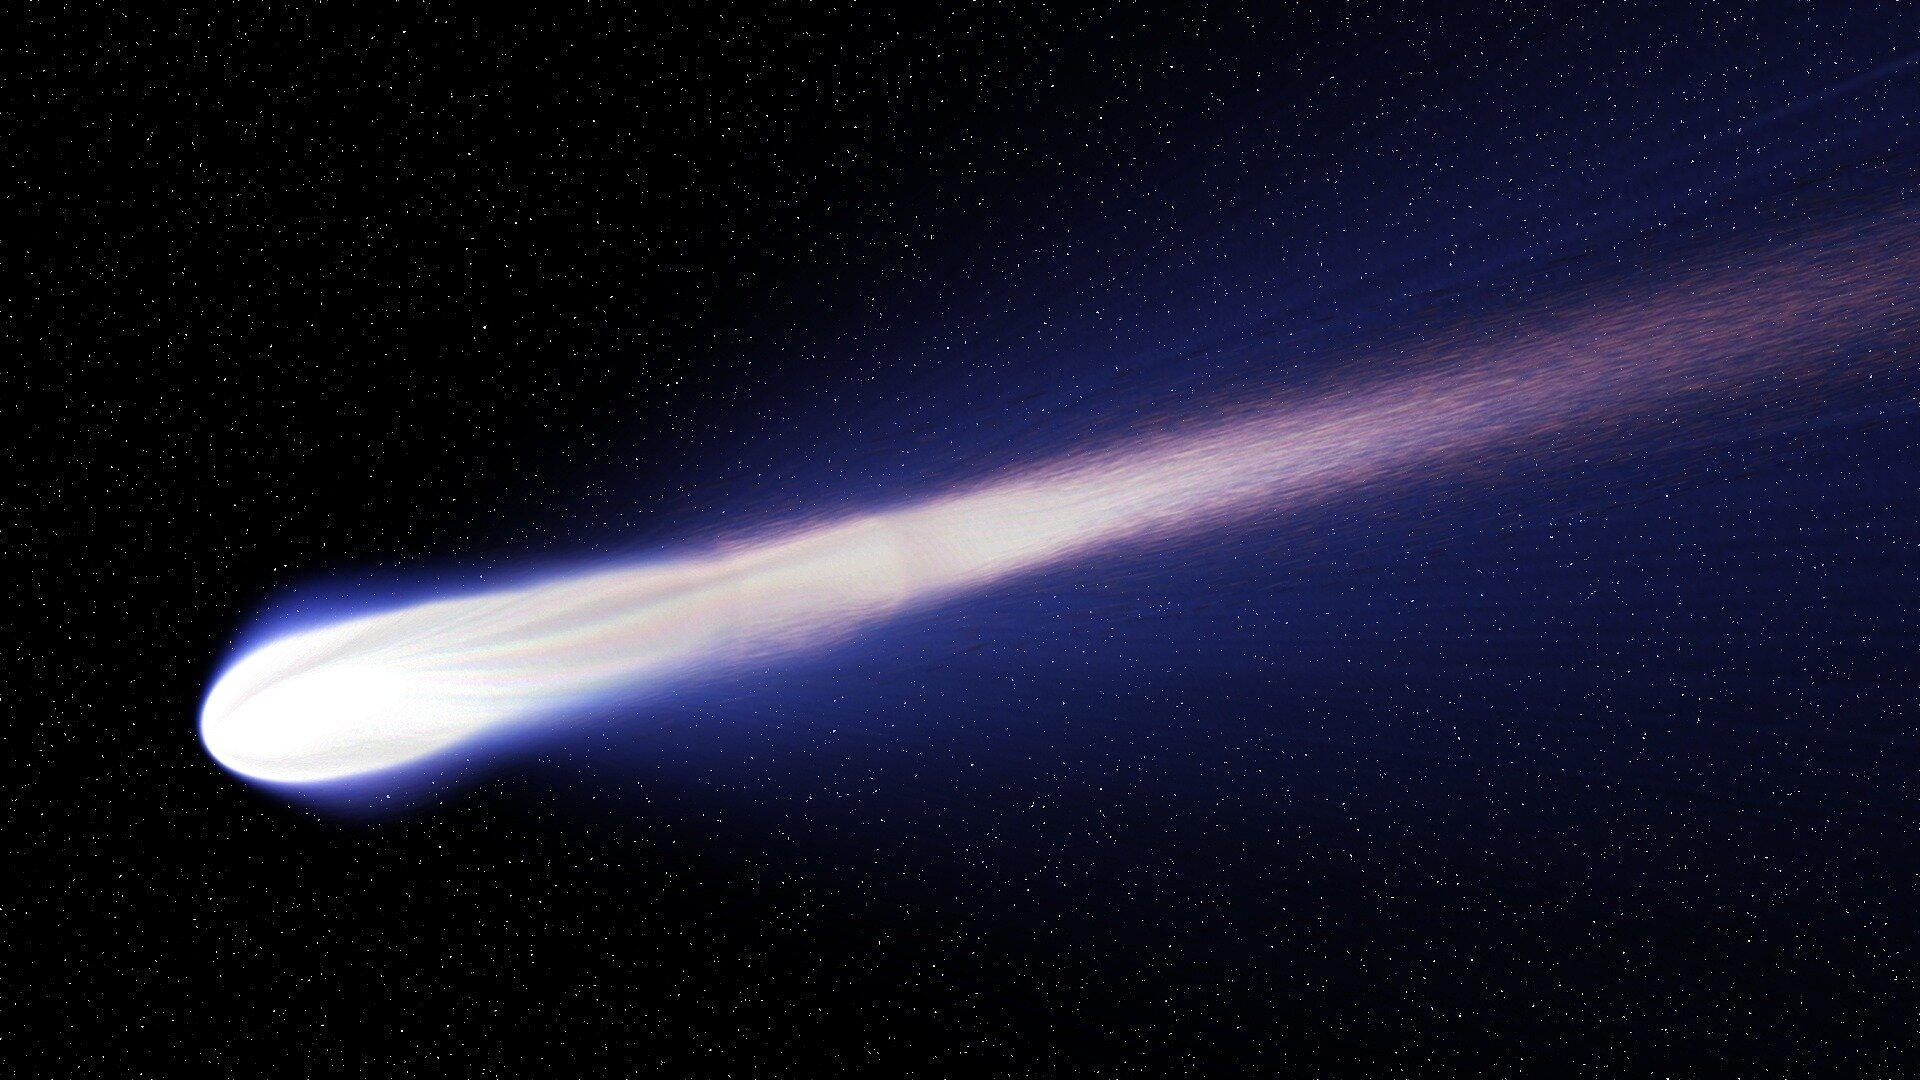
\includegraphics[height=2.75in]{comet.jpg}
\end{frame}
\begin{frame}[fragile]{Shooting Star}
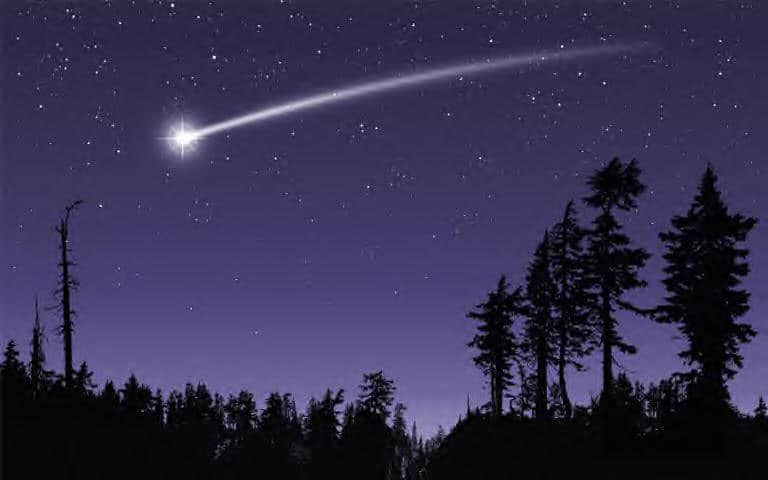
\includegraphics[height=2.75in]{shooting-star-1756306537.jpg}
\end{frame}
\begin{frame}[fragile]{The circuit diagram}
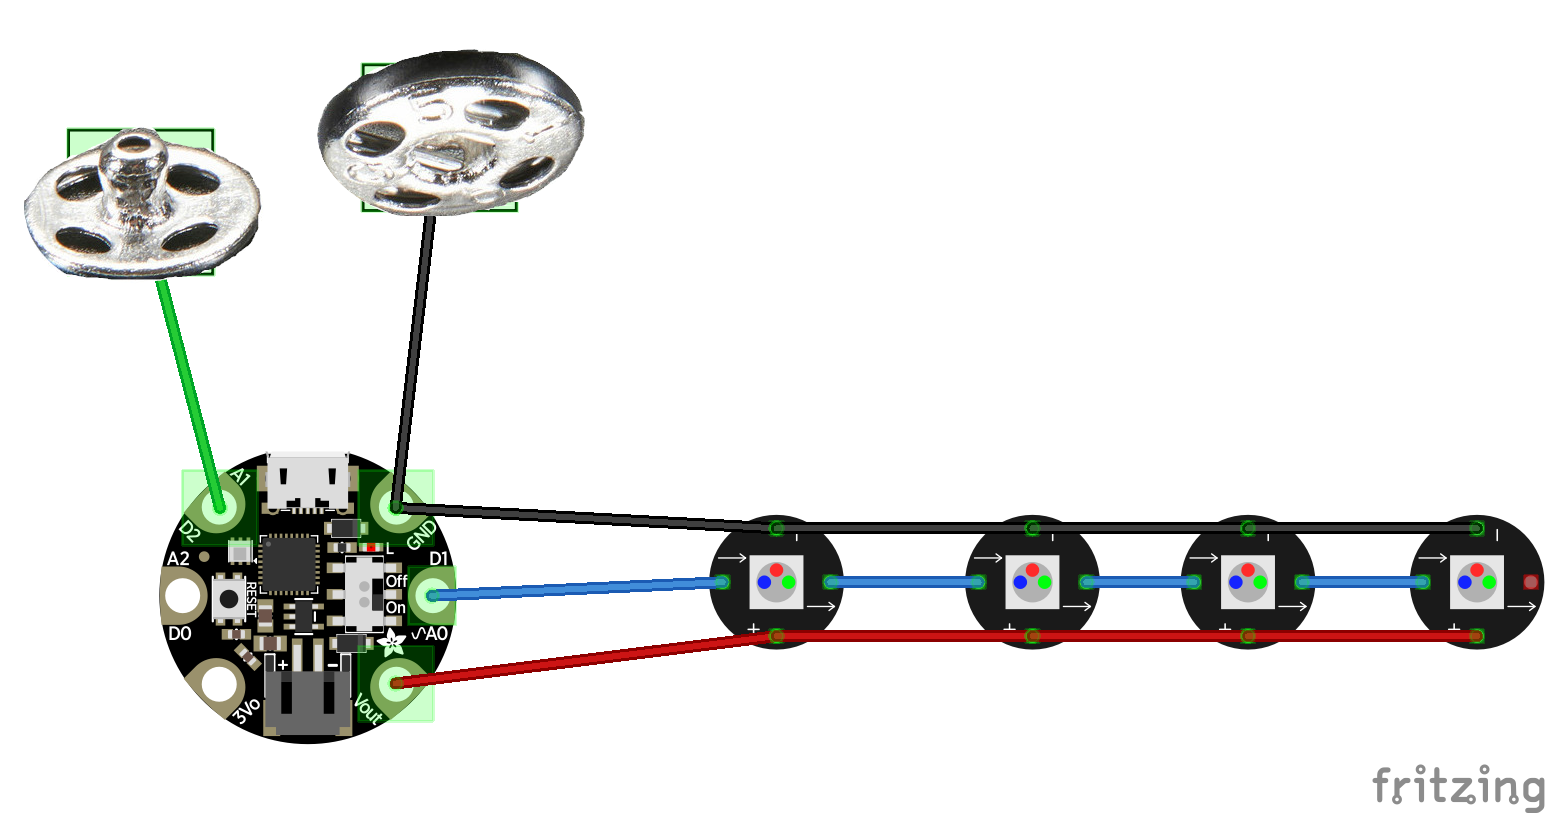
\includegraphics[width=4in]{CircuitDiagram_bb.png}
\end{frame}
\part{Sewing with counductive thread}
\section{''Wiring'' the circuit with conductive thread}
\frame{\tableofcontents[hideothersubsections,sectionstyle=show/hide]}
\subsection{Install the Embroidery Hoop}
\begin{frame}[fragile]{Install the Embroidery Hoop}
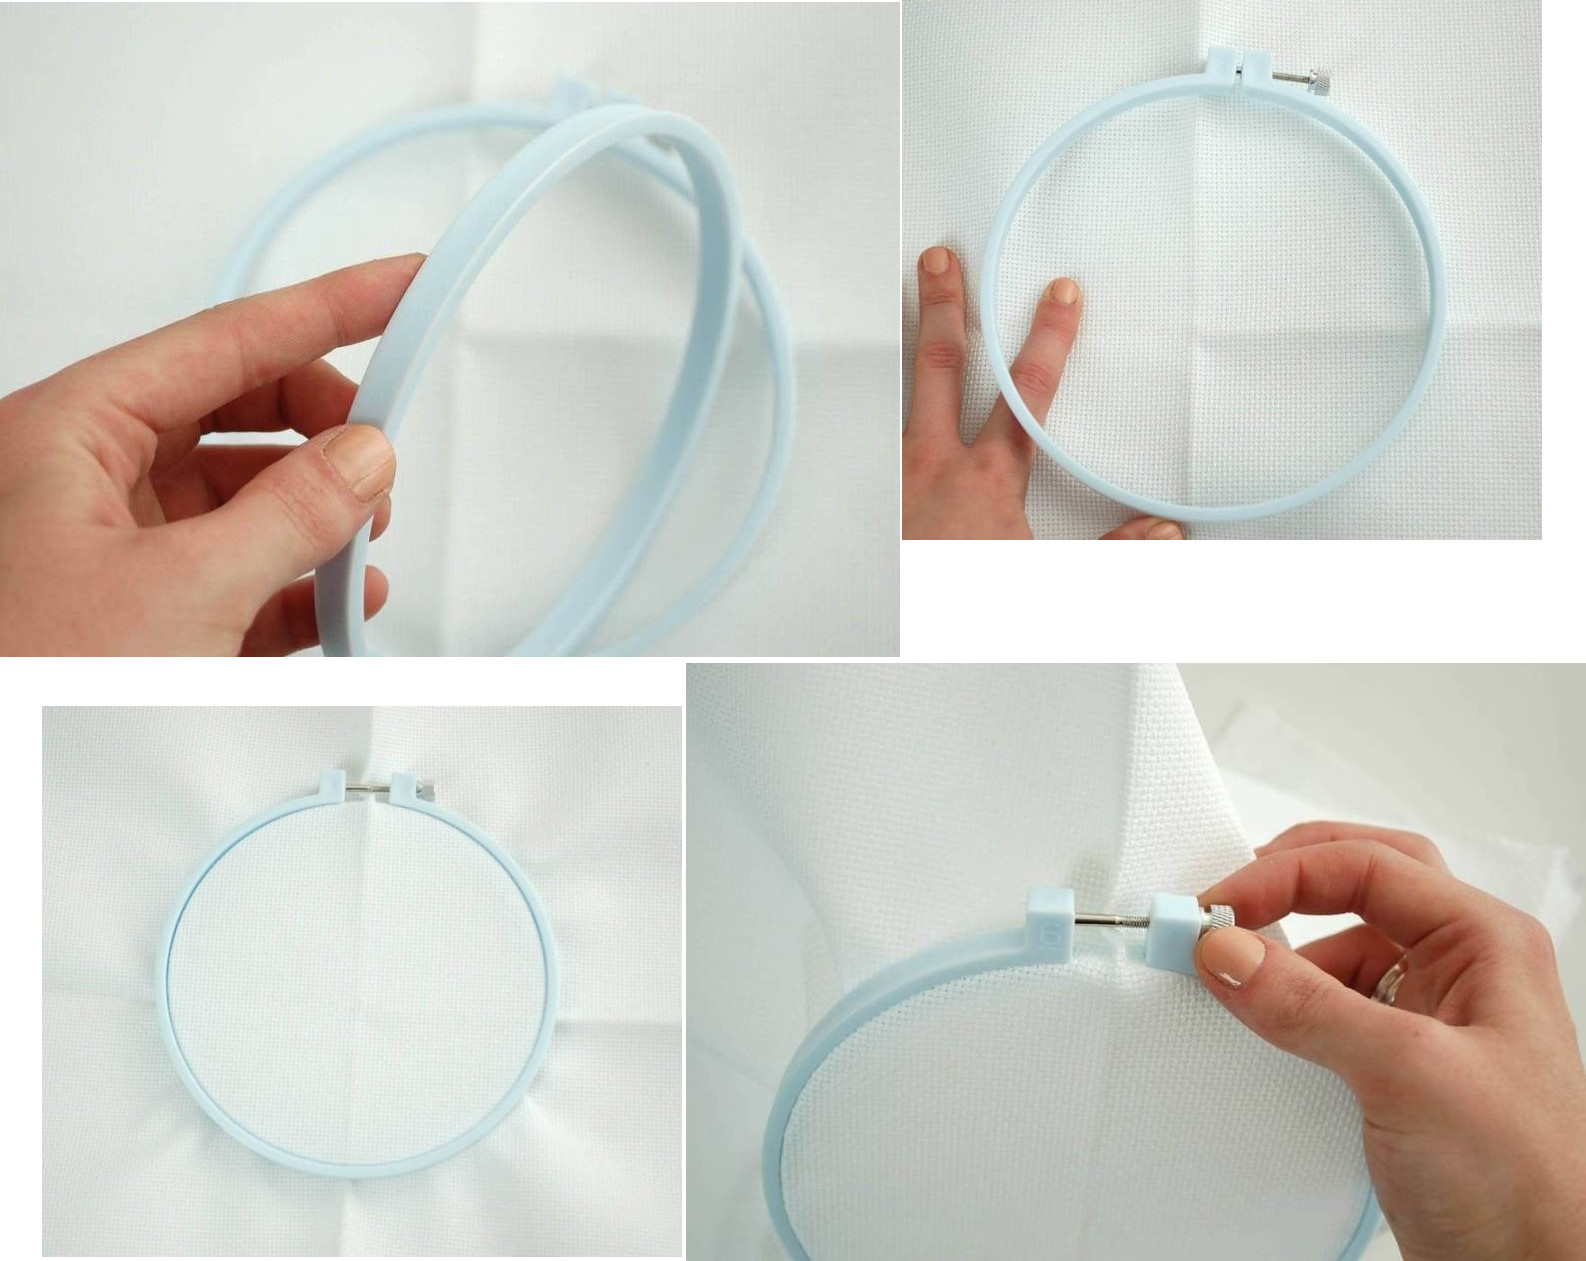
\includegraphics[height=2.75in]{InstallEmbroideryHoop.jpg}
\end{frame} 
\subsection{Wiring the GND wire}
\begin{frame}[fragile]{Wiring the the GND wire}
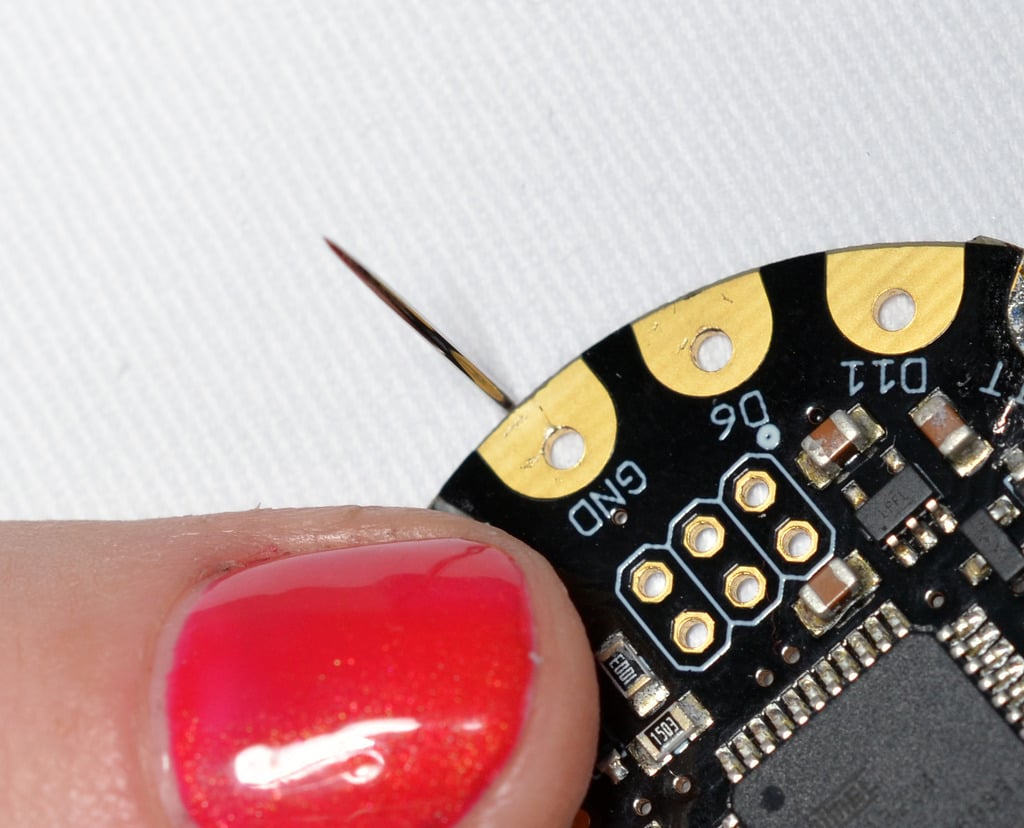
\includegraphics[height=2.75in]{flora_DSC_0099.jpg}
\end{frame}
\begin{frame}[fragile]{Wiring the the GND wire}
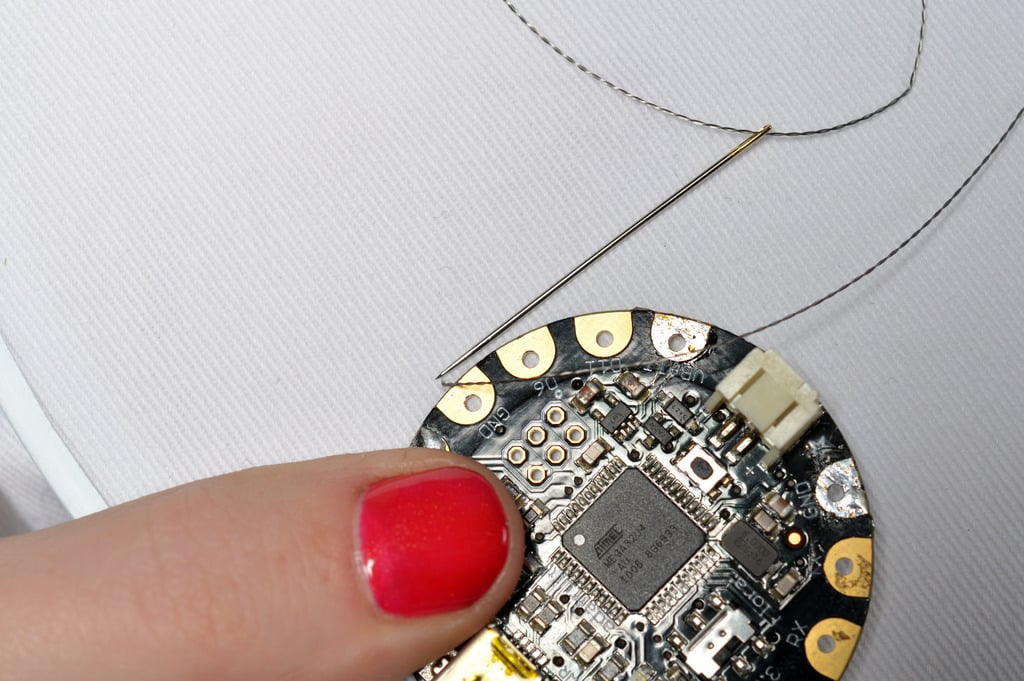
\includegraphics[height=2.75in]{flora_DSC_0100.jpg}
\end{frame}
\begin{frame}[fragile]{Wiring the the GND wire}
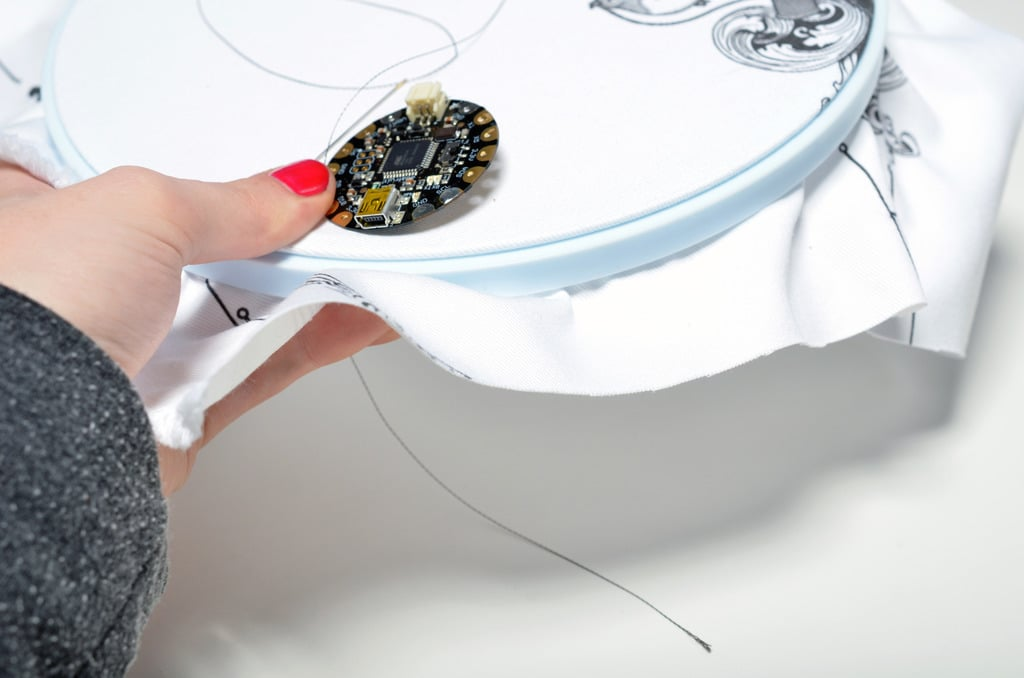
\includegraphics[height=2.75in]{flora_DSC_0101.jpg}
\end{frame}
\begin{frame}[fragile]{Wiring the the GND wire}
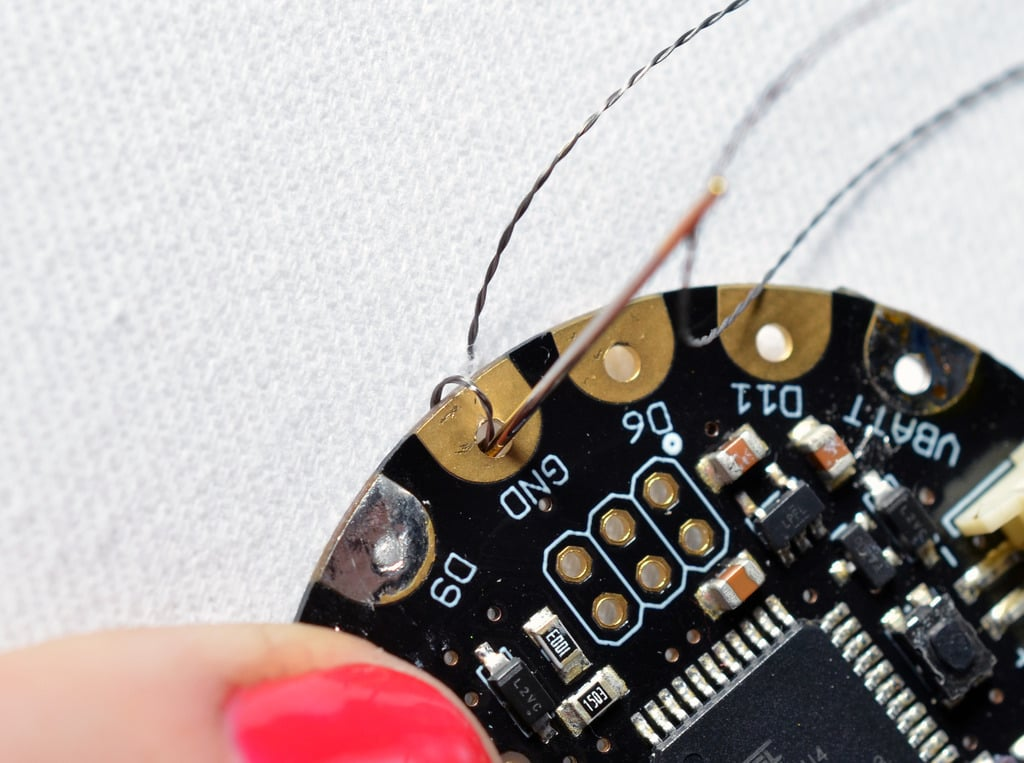
\includegraphics[height=2.75in]{flora_DSC_0103.jpg}
\end{frame}
\begin{frame}[fragile]{Wiring the the GND wire}
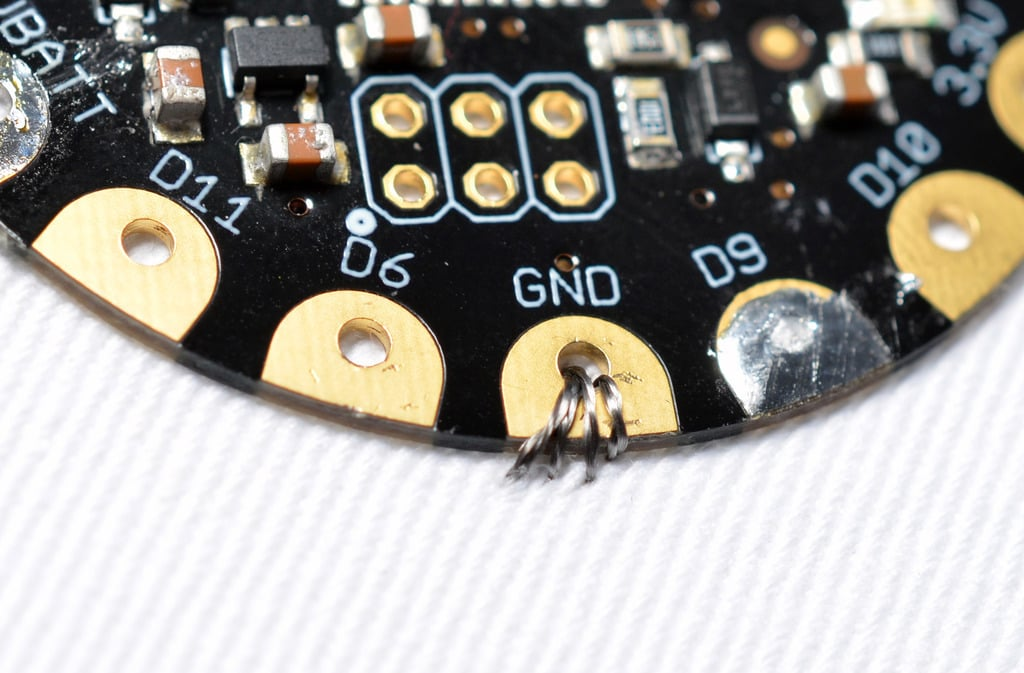
\includegraphics[height=2.75in]{flora_DSC_0105.jpg}
\end{frame}
\begin{frame}[fragile]{Wiring the the GND wire}
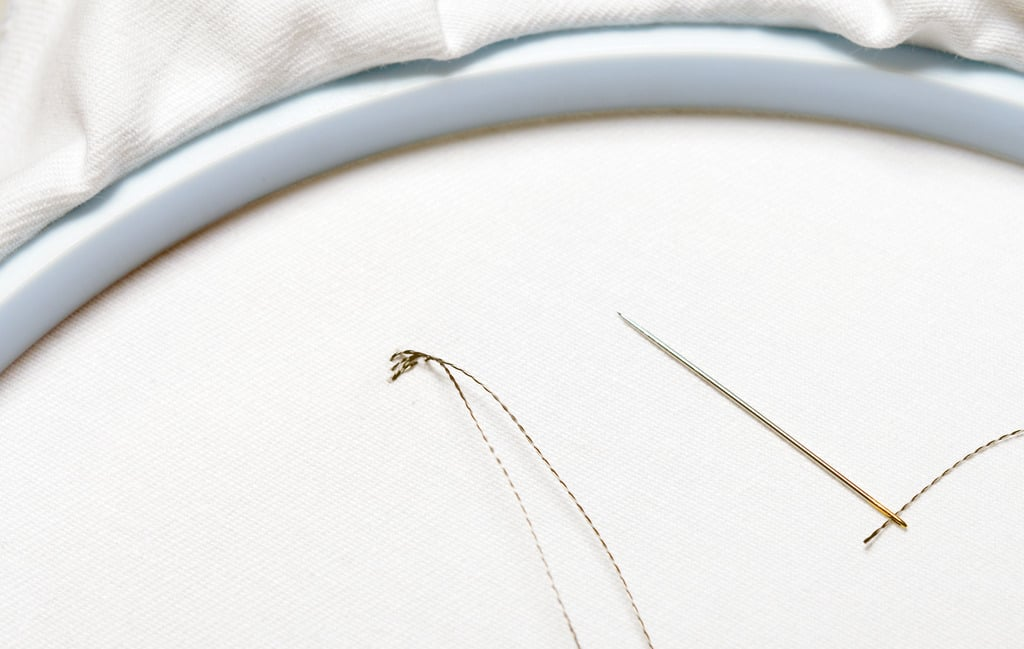
\includegraphics[height=2.75in]{flora_DSC_0106.jpg}
\end{frame}
\begin{frame}[fragile]{Wiring the the GND wire}
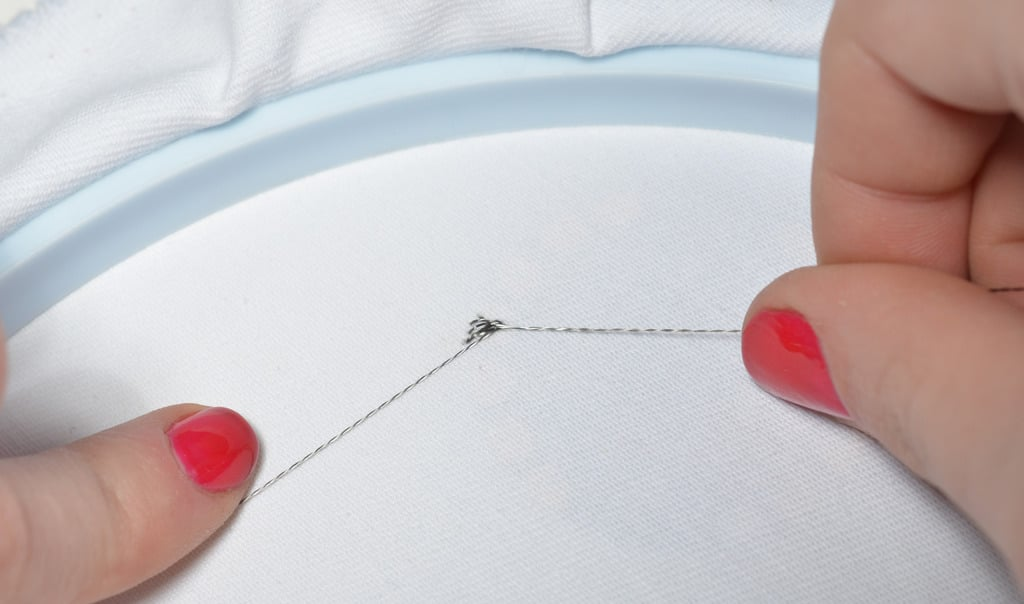
\includegraphics[height=2.75in]{flora_DSC_0107.jpg}
\end{frame}
\begin{frame}[fragile]{Wiring the the GND wire}
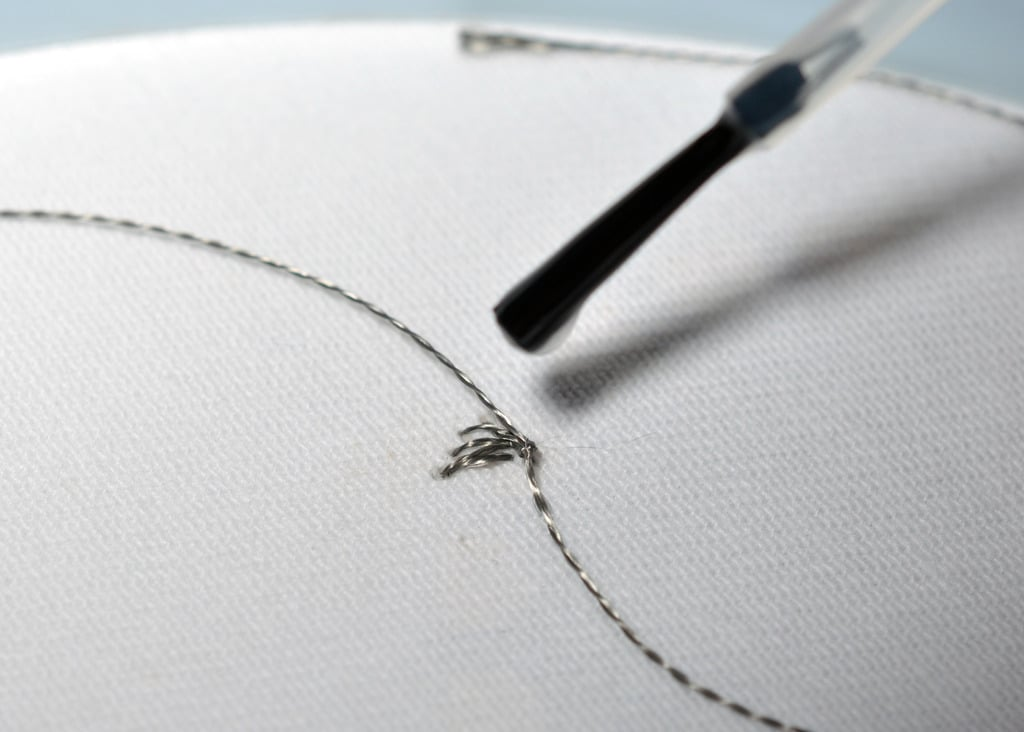
\includegraphics[height=2.75in]{flora_DSC_0109.jpg}
\end{frame}
\begin{frame}[fragile]{Wiring the the GND wire}
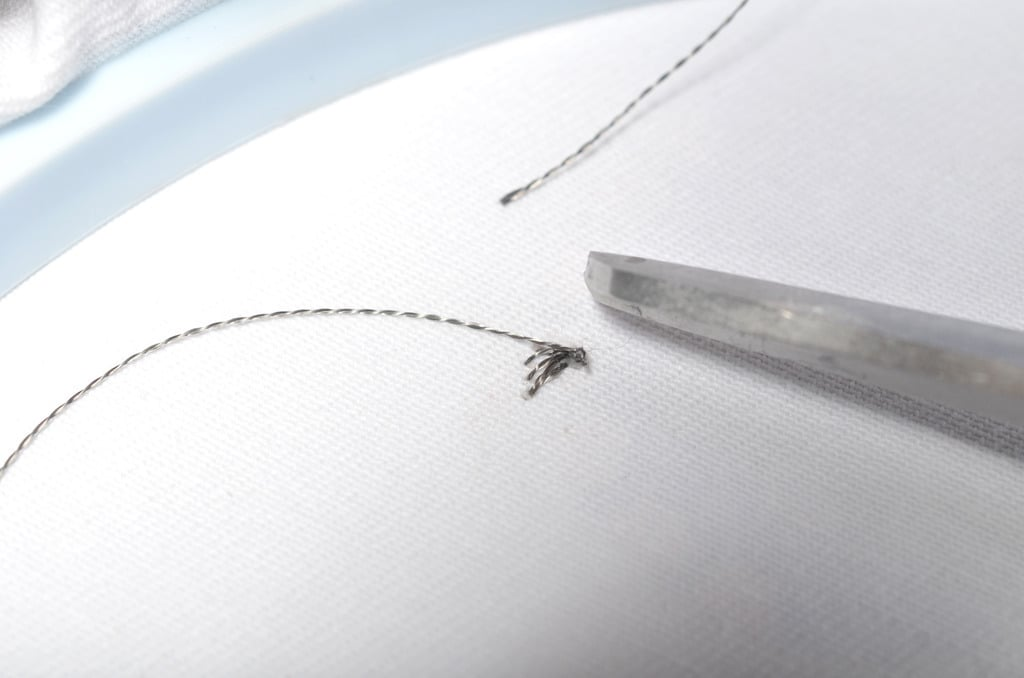
\includegraphics[height=2.75in]{flora_DSC_0111.jpg}
\end{frame}
\begin{frame}[fragile]{Wiring the the GND wire}
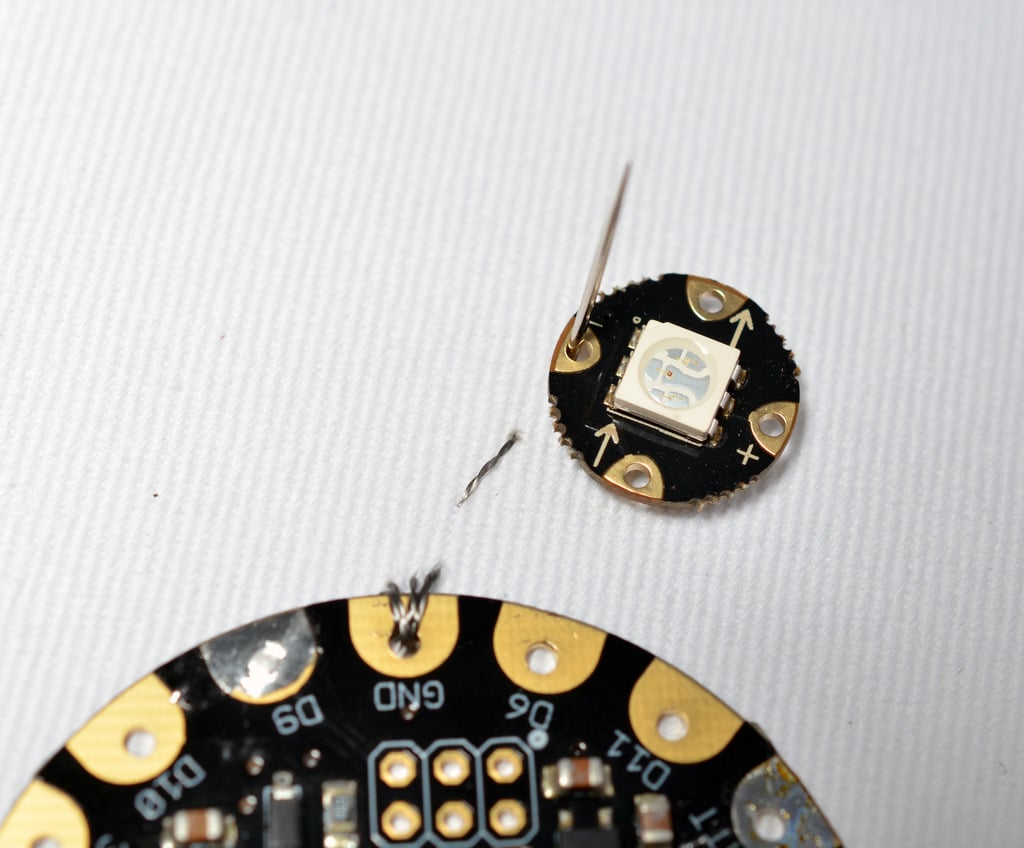
\includegraphics[height=2.75in]{flora_DSC_0113.jpg}
\end{frame}
\begin{frame}[fragile]{Wiring the the GND wire}
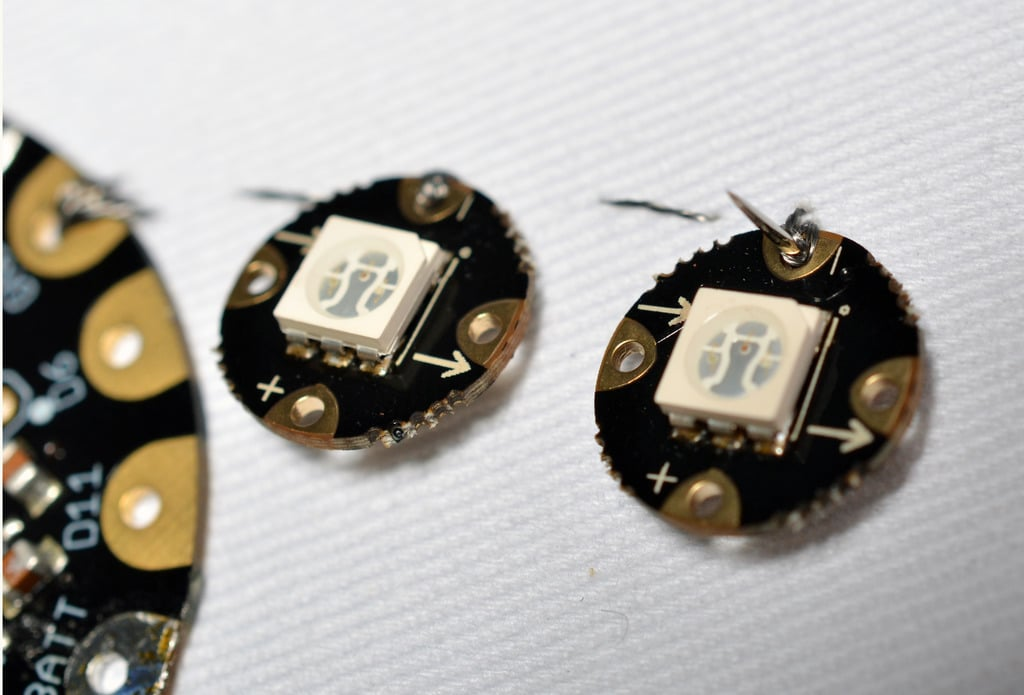
\includegraphics[height=2.75in]{flora_DSC_0115.jpg}
\end{frame}
\begin{frame}[fragile]{Wiring the the GND wire}
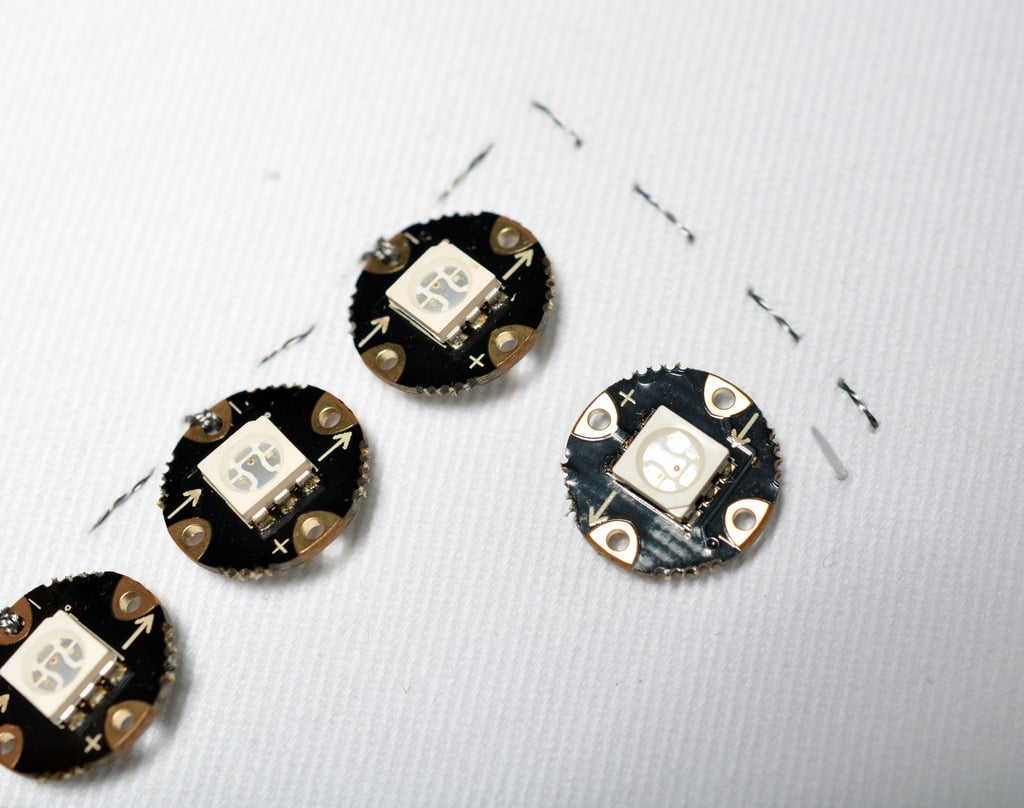
\includegraphics[height=2.75in]{flora_DSC_0116.jpg}
\end{frame}
\begin{frame}[fragile]{Wiring the the GND wire}
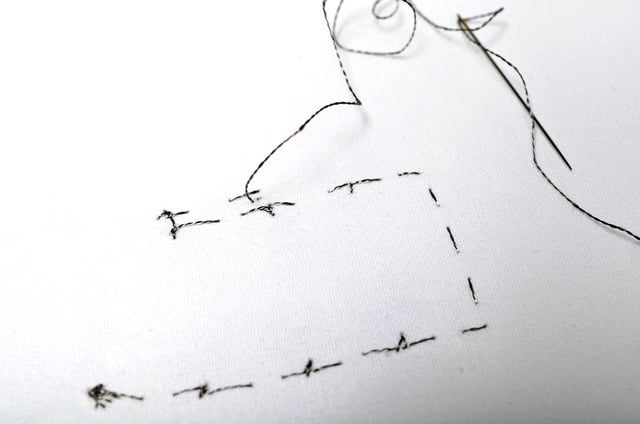
\includegraphics[height=2.75in]{flora_DSC_0118.jpg}
\end{frame}
\begin{frame}[fragile]{Wiring the the GND wire}
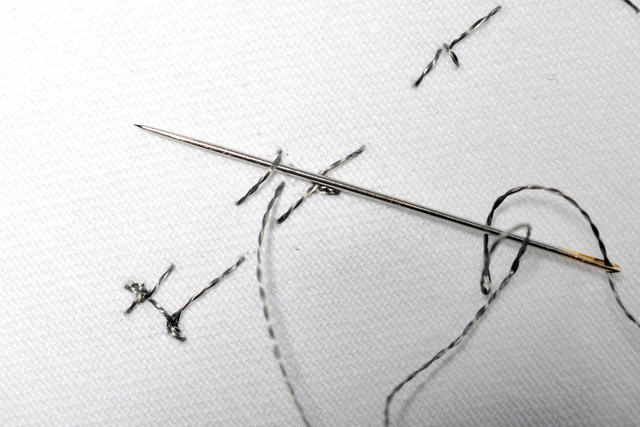
\includegraphics[height=2.75in]{flora_DSC_0119.jpg}
\end{frame}
\begin{frame}[fragile]{Wiring the the GND wire}
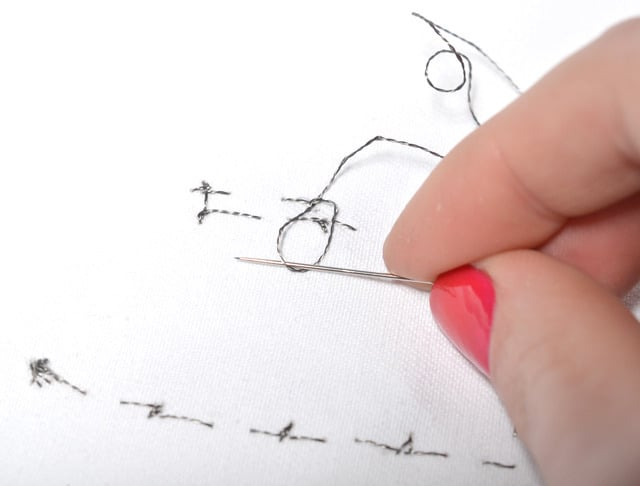
\includegraphics[height=2.75in]{flora_DSC_0120.jpg}
\end{frame}
\begin{frame}[fragile]{Wiring the the GND wire}
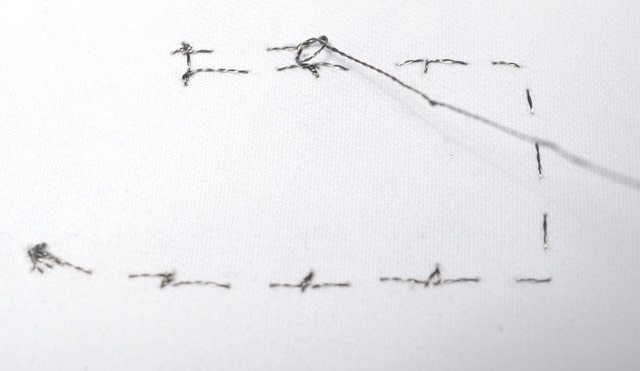
\includegraphics[height=2.75in]{flora_DSC_0121.jpg}
\end{frame}
\begin{frame}[fragile]{Wiring the the GND wire}
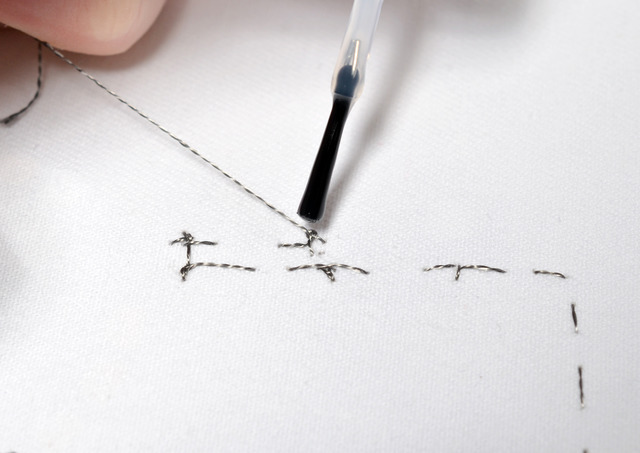
\includegraphics[height=2.75in]{flora_DSC_0123.jpg}
\end{frame}
\begin{frame}[fragile]{Wiring the the GND wire}
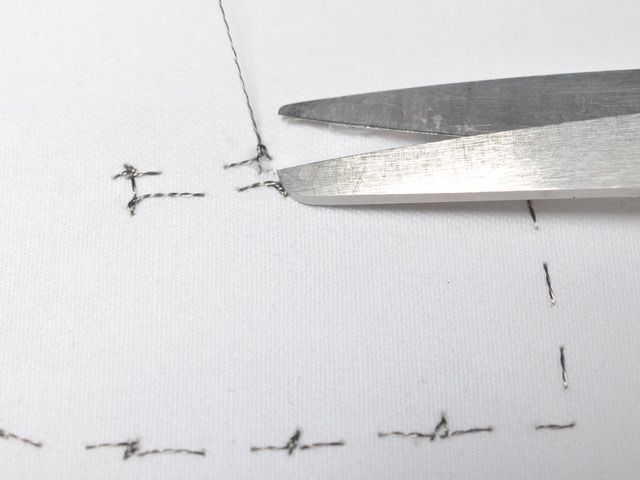
\includegraphics[height=2.75in]{flora_DSC_0125.jpg}
\end{frame}
\subsection{Snap Switch}
\begin{frame}[fragile]{Snap Switch}
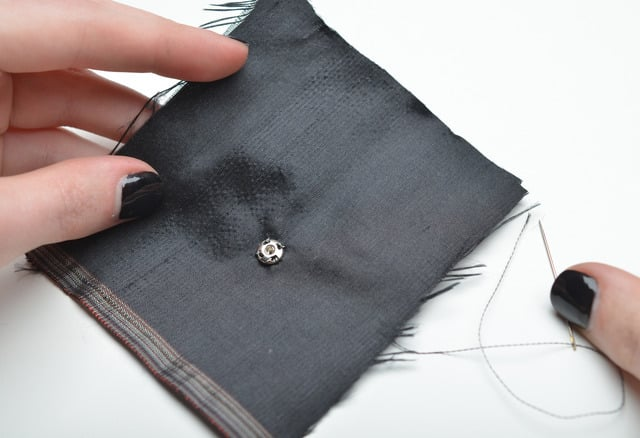
\includegraphics[height=2.75in]{flora-angler-embroidery-17.jpg}
\end{frame}
\begin{frame}[fragile]{Snap Switch}
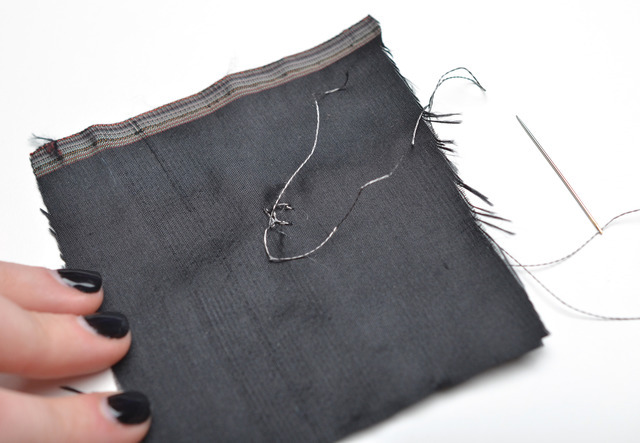
\includegraphics[height=2.75in]{flora-angler-embroidery-18.jpg}
\end{frame}
\begin{frame}[fragile]{Snap Switch}
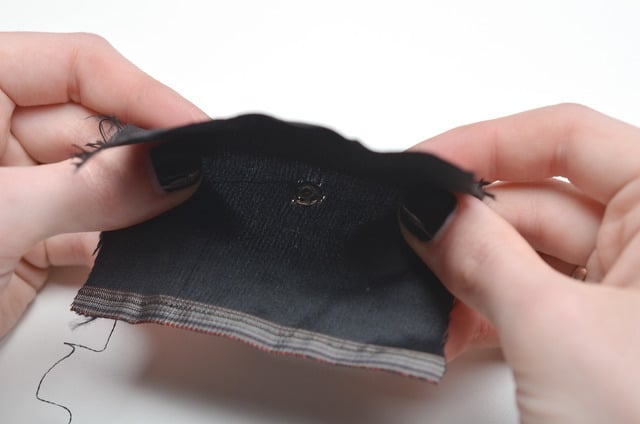
\includegraphics[height=2.75in]{flora-angler-embroidery-19.jpg}
\end{frame}
\begin{frame}[fragile]{Snap Switch}
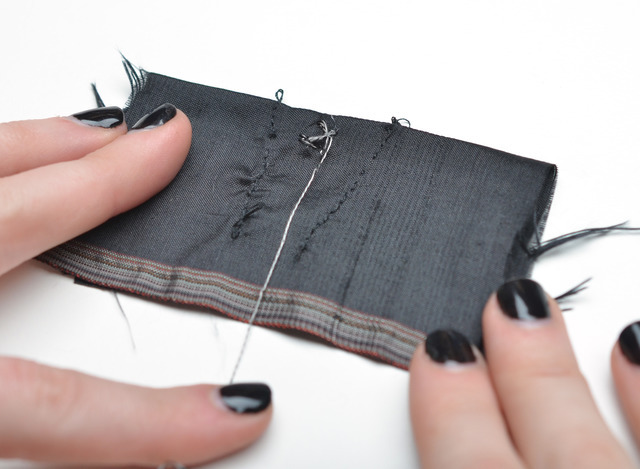
\includegraphics[height=2.75in]{flora-angler-embroidery-20.jpg}
\end{frame}
\begin{frame}[fragile]{Snap Switch}
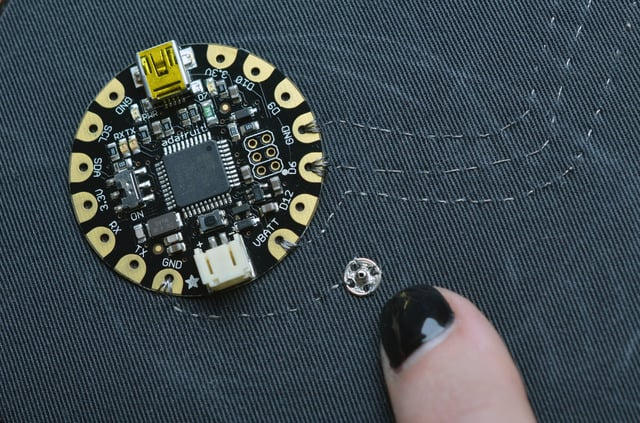
\includegraphics[height=2.75in]{flora-angler-embroidery-21a.jpg}
\end{frame}
\begin{frame}[fragile]{Snap Switch}
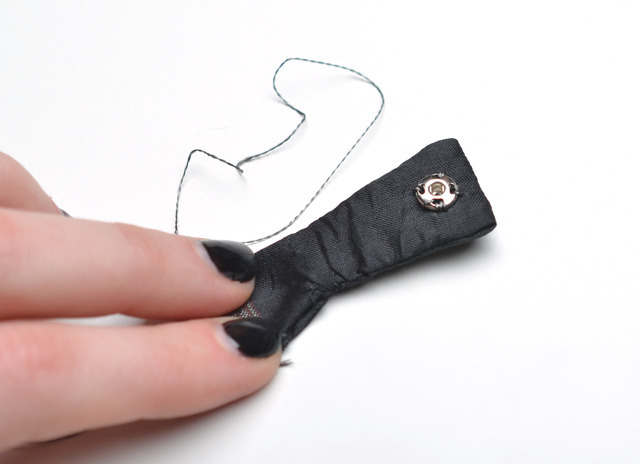
\includegraphics[height=2.75in]{flora-angler-embroidery-21.jpg}
\end{frame}
\begin{frame}[fragile]{Snap Switch}
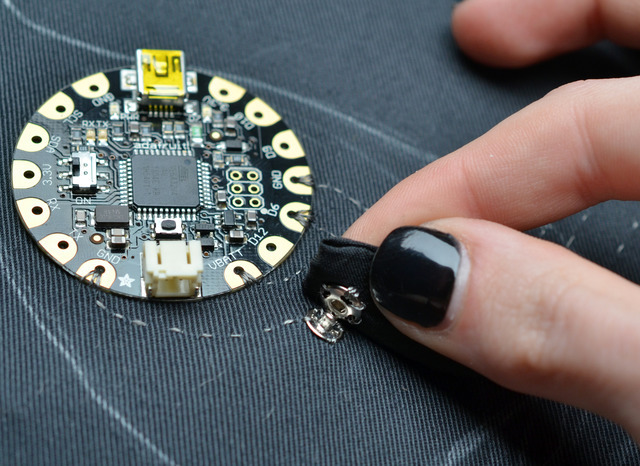
\includegraphics[height=2.75in]{flora-angler-embroidery-22.jpg}
\end{frame}
\begin{frame}[fragile]{Snap Switch}
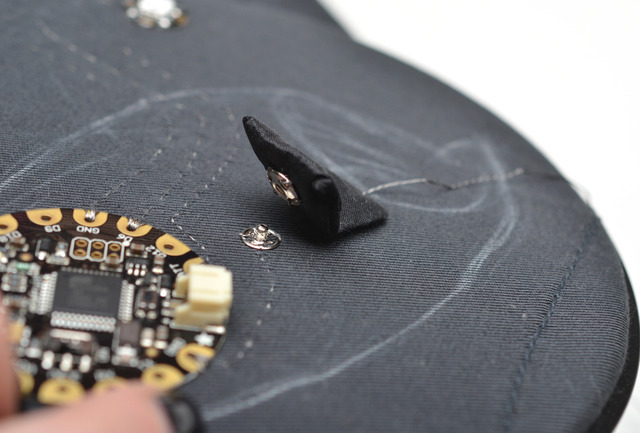
\includegraphics[height=2.75in]{flora-angler-embroidery-23.jpg}
\end{frame}
\begin{frame}[fragile]{Snap Switch}
\includegraphics[height=2.75in]{flora-angler-embroidery-24.jpg}
\end{frame}
\part{Writing the CircuitPython code}
\begin{frame}[fragile]{CircuitPython code}
\lstinputlisting[lastline=17]{RailroadCrossing.py}
\end{frame}
\begin{frame}[fragile]{CircuitPython code}
\lstinputlisting[firstline=18]{RailroadCrossing.py}
\end{frame}
\end{document}
